\documentclass[]{article}
\usepackage{lmodern}
\usepackage{amssymb,amsmath}
\usepackage{ifxetex,ifluatex}
\usepackage{fixltx2e} % provides \textsubscript
\ifnum 0\ifxetex 1\fi\ifluatex 1\fi=0 % if pdftex
  \usepackage[T1]{fontenc}
  \usepackage[utf8]{inputenc}
\else % if luatex or xelatex
  \ifxetex
    \usepackage{mathspec}
  \else
    \usepackage{fontspec}
  \fi
  \defaultfontfeatures{Ligatures=TeX,Scale=MatchLowercase}
\fi
% use upquote if available, for straight quotes in verbatim environments
\IfFileExists{upquote.sty}{\usepackage{upquote}}{}
% use microtype if available
\IfFileExists{microtype.sty}{%
\usepackage{microtype}
\UseMicrotypeSet[protrusion]{basicmath} % disable protrusion for tt fonts
}{}
\usepackage[margin=1in]{geometry}
\usepackage{hyperref}
\hypersetup{unicode=true,
            pdftitle={Project Report},
            pdfauthor={Sameera Suhail},
            pdfborder={0 0 0},
            breaklinks=true}
\urlstyle{same}  % don't use monospace font for urls
\usepackage{longtable,booktabs}
\usepackage{graphicx,grffile}
\makeatletter
\def\maxwidth{\ifdim\Gin@nat@width>\linewidth\linewidth\else\Gin@nat@width\fi}
\def\maxheight{\ifdim\Gin@nat@height>\textheight\textheight\else\Gin@nat@height\fi}
\makeatother
% Scale images if necessary, so that they will not overflow the page
% margins by default, and it is still possible to overwrite the defaults
% using explicit options in \includegraphics[width, height, ...]{}
\setkeys{Gin}{width=\maxwidth,height=\maxheight,keepaspectratio}
\IfFileExists{parskip.sty}{%
\usepackage{parskip}
}{% else
\setlength{\parindent}{0pt}
\setlength{\parskip}{6pt plus 2pt minus 1pt}
}
\setlength{\emergencystretch}{3em}  % prevent overfull lines
\providecommand{\tightlist}{%
  \setlength{\itemsep}{0pt}\setlength{\parskip}{0pt}}
\setcounter{secnumdepth}{5}
% Redefines (sub)paragraphs to behave more like sections
\ifx\paragraph\undefined\else
\let\oldparagraph\paragraph
\renewcommand{\paragraph}[1]{\oldparagraph{#1}\mbox{}}
\fi
\ifx\subparagraph\undefined\else
\let\oldsubparagraph\subparagraph
\renewcommand{\subparagraph}[1]{\oldsubparagraph{#1}\mbox{}}
\fi

%%% Use protect on footnotes to avoid problems with footnotes in titles
\let\rmarkdownfootnote\footnote%
\def\footnote{\protect\rmarkdownfootnote}

%%% Change title format to be more compact
\usepackage{titling}

% Create subtitle command for use in maketitle
\providecommand{\subtitle}[1]{
  \posttitle{
    \begin{center}\large#1\end{center}
    }
}

\setlength{\droptitle}{-2em}

  \title{Project Report}
    \pretitle{\vspace{\droptitle}\centering\huge}
  \posttitle{\par}
    \author{Sameera Suhail}
    \preauthor{\centering\large\emph}
  \postauthor{\par}
      \predate{\centering\large\emph}
  \postdate{\par}
    \date{6/12/2019}

\usepackage{setspace}
% this is a lorem ipsum generator for adding dummy texts
\usepackage{lipsum}
\usepackage{tocloft}
% to make the first rows bold in tables
\usepackage{longtable}
\usepackage{tabu}
\usepackage{booktabs}
% this makes list of figures appear in table of contents
\usepackage[nottoc]{tocbibind}

% for passing temporary notes
\usepackage{todonotes}

\usepackage{morefloats}
\usepackage{float}

% highlighting
\usepackage{soul}

% referencing mutliple things with a single command - \cref
\usepackage{cleveref}


% this makes dots in table of contents
\renewcommand{\cftsecleader}{\cftdotfill{\cftdotsep}}
% to change the title of contents
% \renewcommand{\contentsname}{Whatever}

% line numbers for review purposes
% this package might not be available in default latex installation 
% get it by 'sudo tlmgr install lineno'
%\usepackage{lineno}
%\linenumbers

% this allows checkmarks in the file
\usepackage{amssymb}
\DeclareUnicodeCharacter{2714}{\checkmark}

% to be able to include latex comments
\newenvironment{dummy}{}{}
\usepackage{booktabs}
\usepackage{longtable}
\usepackage{array}
\usepackage{multirow}
\usepackage{wrapfig}
\usepackage{float}
\usepackage{colortbl}
\usepackage{pdflscape}
\usepackage{tabu}
\usepackage{threeparttable}
\usepackage{threeparttablex}
\usepackage[normalem]{ulem}
\usepackage{makecell}
\usepackage{xcolor}

\widowpenalties 1 150 \usepackage{float} \floatplacement{figure}{H} \floatplacement{table}{H}

\begin{document}
\maketitle


\onehalfspacing
\pagenumbering{gobble}

%\begin{titlepage}
\begin{center}
\vspace*{2\baselineskip}
\LARGE{\textbf{Artificial Neural Network Based Modelling of Organic Photovoltaic Cells}}\\
\vspace*{1\baselineskip}
\vspace*{2\baselineskip}
\Large{\textbf{Major Research Project }}\\
\Large{\textbf{EEE80018 }}\\
\vspace*{2\baselineskip}
\vspace*{2\baselineskip}
\Large{Sameera Suhail}\\
\Large{Student ID: 101739677}\\
\vspace*{1\baselineskip}
\vspace*{2\baselineskip}
\vspace*{3\baselineskip}
\Large{\textbf{Project Supervisor}}\\
Dr. Jagdish Patra\\
\end{center}
% \end{titlepage}

\doublespacing


\hypersetup{linkcolor = black}
\newpage
\pagenumbering{roman}
\tableofcontents
\addcontentsline{toc}{section}{\contentsname}


\doublespacing

\newpage
\pagenumbering{arabic}
\hypersetup{linkcolor = blue}


\doublespacing


%\begin{abstractpage}
\begin{center}
\Large{\textbf{Abstract}}\\
\end{center}
\normalsize{Even though Organic Photovoltaic Cells (OPV) have been around since 1980s, their use was limited due
to their low efficiencies. With these efficiencies now on the rise, they have become commercially relevant.
The present study is based on OPVs that have poly(3,4-ethylenedioxythiophene):poly(styrenesulfonate)
(PEDOT:PSS) as a hole extracting layer (HEL) and anionic fluorinated ionomers (PFI) as additives in
the HEL. Analytical modeling of solar cell characteristics is difficult and to some extent inaccurate as
many assumptions have to be made. We, therefore, attempt to use Artificial Neural Networks (ANN) in the
case of OPVs with PFI in PEDOT:PSS layer to model two characteristics of OPVs: one optical and one
electrical. Use of multilayer perceptrons along with functional link neural networks allows for comparison
of both ANNs in terms of both training times and accuracies. The accuracies obtained with both MLP
and FLANN are close to each other but, as expected, FLANN trains faster.}\\
%\end{abstractpage}

\doublespacing

\newpage

\newpage

\hypertarget{introduction}{%
\section{Introduction}\label{introduction}}

In recent years, organic photovoltaics (OPVs) have become popular due to their low cost, easy manufacturing, high flexibility and high absorption coefficients. They don't require high-temperature vacuum processes for manufacturing which makes it possible to produce them in bulk, using methods such as spin-coating, ink-jet printing, spray deposition and roll-to-roll processing {[}1{]}--{[}12{]}. Despite the many benefits of adopting OPVs commercially, their use remains limited due to their low efficiency and stability. Till 2018, OPVs with efficiencies greater than 10\% have been reported{[}13{]}--{[}17{]}. The degradation mechanisms responsible for low lifetimes of OPVs are environmental factors such as exposure to \(O_2\) and \(H_2O\), photochemical and metal ion diffusion from the electrodes.

The functioning of an organic solar cell includes a number of steps. Firstly, under illumination, a photon is absorbed by the active layer leading to the formation of an electron-hole pair. The pair (exciton) is then separated and the electrons go towards cathode and the holes go towards anode. This means that the cathode is supposed to have lower work functions to attract the electrons while the anode is supposed to have higher work functions to attract the holes. The current, therefore, flows out of the anode side of the photovoltaic cell and into the cathode. Ideally, the contact resistance at the electrode interfaces determines the device photovoltage. The smaller the resistance, the smaller is the barrier that the charges experience at the electrodes. Additional layers are included between the active layer and each electrode to modify their work functions. LiF is a common material that reduces the work function of the cathode by being used between the metal cathode and the active layer {[}18{]}. Similarly, poly(3,4-ethylenedioxythiophene):poly(styrenesulfonate) (PEDOT:PSS) increases the work function of the anode side of the cell and helps in reducing the injection barrier experienced by the holes{[}19{]}.

Therefore, the PEDOT:PSS layer sitting between the Titanium Indium oxide anode and the active layer is called a Hole Extraction Layer (HEL). It has applications in other organic optoelectronic devices and is cheap, environmentally friendly and easily manufactured without requiring high temperature processing. The conducting polymer has large ionization potential, high conductivity and large transparency. The transparency ensures that light reaches the active layer where the disassociation of excitons actually occurs.

PEDOT:PSS, however, has its own share of issues. Its high chemical reactivity makes the cell susceptible to degradation due to environmental factors {[}20{]}. Its electronic properties are modified for the worse when the hygroscopic layer absorbs moisture and its work function reduces towards vacuum, thereby, decreasing the charge extraction capacity of the OPV. In the study by Howells et al.~{[}21{]} anionic fluorinated ionomers (PFI) were used as additives in the PEDOT:PSS layer. The advantage attained from doing so was twofold: first to reduce degradation of OPV from \(H_2O\) and \(O_2\); second to tune its work function to higher values leading to better charge extraction. Different concentrations of PFI were experimented with in the study at hand {[}21{]}. Although, the effect of PFI concentration was studied on a number of OPV characteristics, in this study I attempted to use Neural Networks to model only the transmittance as a function of light wavelength and the J-V characteristics at 0 hour of continuous AM1.5 G illumination at 100mW cm-2.
The rest of the report has been divided into a number of sections. Section 2 gives an overview of the development of OPVs since their discovery and the use of neural networks in past researches involving modeling of solar cell characteristics. Section 3 describes briefly the two different types of ANN that will be employed in this study and the design of experiments. Section 4 shows the analysis and results obtained. Finally section 5 gives the concluding remarks on the results and implications.

\hypertarget{literature-review}{%
\section{Literature Review}\label{literature-review}}

The very first OPVs consisted of a single organic layer between two metal electrodes having different work functions{[}22{]}, {[}23{]}. Then in 1986, heterojunction bilayers came to the scene where two layers having n-type and p-type properties respectively were sandwiched between the two electrodes {[}24{]}. As more research led to the development of conjugated polymers, OPVs with polymer-fullerene bulk heterojunction became popular {[}25{]}, {[}26{]}. The most widely used one is P3HT:PC61BM bulk heterojunction, where PC61BM is a fullerene derivative acceptor with high electron affinity and P3HT is a polymer donor with high ionization potential. The aim of bulk heterojunction is to intermix the acceptor and donor polymers in bulk in order to increase the area for charge separation to occur. This ensures that recombination stays to a minimum and all excitons are disassociated. The aforementioned P3HT:PC61BM devices are made using solution casting of P3HT and PC61BM blends {[}27{]}.
Attempts have been made to accurately model the characteristics of OPVs in order to enhance the design of solar cells. Suliman et al.~{[}28{]} achieved optimal device performance using response surface methodology using three variables: polymer concentration, polymer-fullerene ratio and active layer spinning speed. The use of a statistical tools meant the use of complex mathematics. Pillai et al.~{[}29{]} opted to use simple circuit equations of a reverse double diode model to model the behavior of nav-100 an OPV. The unknown parameters in the double diode model were nevertheless extracted using Genetic Algorithm. Fallahpour et al.~{[}30{]} adopted Transfer Matrix Method and Drift Diffusion concept to model the model light absorption and charge transport respectively for energetically disordered solar cells. In such studies involving analytical modeling techniques, results are often obtained after several assumptions and approximations {[}31{]}.

Artificial neural networks (ANNs) have, however, been known to give excellent results in areas involving high noise and non-linear input to output mapping {[}32{]}. The present study is based on the experimental study by Howell et al.~{[}21{]}, where the optoelectronic and topographical properties of PEDOT:PSS with different concentrations of PFI additive were studied. The characteristics studied were transmittance, topography, work function, contact angle with water, J-V device characteristics and degradation studies using Jsc, Voc, Fill Factor (FF), and Power Conversion Efficiency (PCE) as parameters {[}21{]}.

\hypertarget{research-design}{%
\section{Research Design}\label{research-design}}

\hypertarget{experiment-characterization-and-input-dataset}{%
\subsection{Experiment Characterization and Input Dataset}\label{experiment-characterization-and-input-dataset}}

The transmission (T\%) vs.~wavelength (\(\lambda\)) and current density (J) vs.~voltage (V) characteristics were modeled using ANNS. Both characteristics were first modeled using multilayer perceptrons (MLPs) and then functional link neural networks (FLANNs). To decide the best architecture, the number of hidden layers in MLP was restricted to one as the number of features was two at most. The number of neurons in the hidden layer was, however, varied to arrive at the architecture giving the best performance. With regards to FLANN, the polynomial used for functional expansion was varied among Chebyshev, Legendre, Trigonometric and Power. The polynomial with relatively better performance among these four was finally chosen.

\begin{figure}
\centering
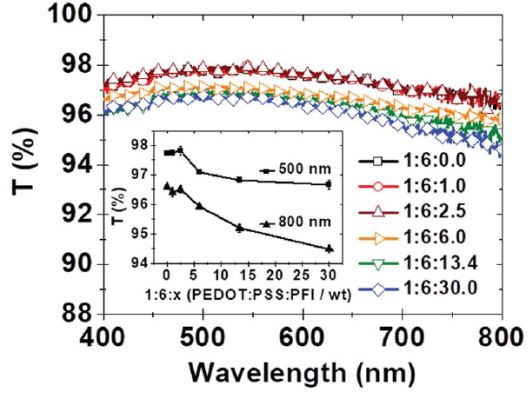
\includegraphics[width=0.5\textwidth,height=\textheight]{images/trans.jpg}
\caption{Transmittance vs.~wavelength \label{fig:transfig}}
\end{figure}

\begin{figure}
\centering
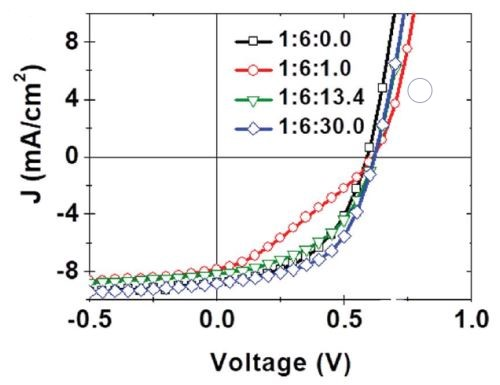
\includegraphics[width=0.5\textwidth,height=\textheight]{images/JV.jpg}
\caption{Current Density vs.~Voltage \label{fig:JVfig}}
\end{figure}

The two characteristics obtained experimentally in the parent study are shown in Figures \ref{fig:transfig} and \ref{fig:JVfig}.

The experiments for each characteristic were divided into two: one with a single input and a single output and the other one with two inputs (second one being the concentration of PFI) and one output.

\begin{figure}
\centering
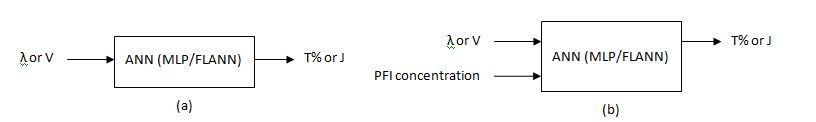
\includegraphics[width=1\textwidth,height=\textheight]{images/block.jpg}
\caption{Experiment Design \label{fig:blocks}}
\end{figure}

Thus, depending on whether the characteristic is T\% vs.~\(\lambda\) or J vs.~V, the experiments were designed as shown in Figure \ref{fig:blocks}.

For the single-input experiments, the ANN is trained and tested using data corresponding to any one PFI concentration. The best-architecture is found using that concentration and the final ANN is used on the data for other concentrations. For the two-input experiments, all available data points are used for training and testing to find the best architecture. To judge the reliability of the final ANN, a new PFI concentration is given to the ANN to predict its transmittance/current density. True output values for this concentration are not known and therefore it is not possible to use performance metrics such as mean absolute error (MAE) etc. to judge its performance numerically. However, the graph corresponding to the new concentration is plotted on the existing figure obtained experimentally. The position of the new line with respect to other concentrations' lines gives a rough idea about the accuracy and reliability of the ANN.

The numbers of samples to ANN for single-input experiments are between 26 and 27, while for two-input experiments they are 100 for J vs.~V and 162 for T\% vs.~\(\lambda\) respectively. In the case of FLANN, each feature was expanded into five features using a polynomial. The relatively low numbers of samples were split for training and testing into 70\% and 30\% of the total samples. This meant that the ANN was trained with as low as 19 samples. This limited the ANN from having a vast pool of examples to learn from.

\hypertarget{multilayer-perceptron}{%
\subsection{Multilayer Perceptron}\label{multilayer-perceptron}}

Multilayer perceptrons are neural networks with one or more hidden layers between the input layer and output layer. Each layer is composed of a number of nodes or neurons which are processing units for the data they receive from the previous layer. The input layer doesn't have a preceding layer and therefore accepts the data samples directly and has neurons equal to the number of features in the dataset. The neurons in the subsequent layers are connected to the previous layers' neurons with connecting links, each associated with a number called weight. The weight multiples the output of a neuron and gives the multiplied value as an input to the next neuron, which then modifies the input according to its activation function.

\begin{figure}
\centering
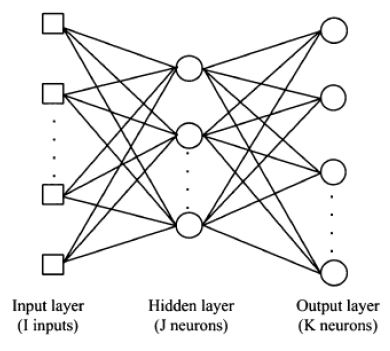
\includegraphics[width=0.5\textwidth,height=\textheight]{images/mlp.jpg}
\caption{Multilayer Perceptron \label{fig:mlp}}
\end{figure}

Figure \ref{fig:mlp} shows the general architecture of an ANN. A fully connected neuron network has no broken links between any two layers. The more number of features and more complex the pattern to be learned, the greater number of layers and neurons may be required.
The neural network learns during the training phase where it accepts the training samples and outputs the predicted values using a set of randomly assigned weights. The predicted values are compared with the true values and the errors are used to slightly modify the weights. The network again outputs some values to be compared with true values, and to be used to again modify the weights in the direction of error reduction. This iterative process employs back propagation algorithm and stops when the network has converged i.e.~the predicted and true values come sufficiently close numerically.

A number of training algorithms exist that can optimize the performance function. These optimizers are based on either the gradient of network performance or the Jacobian of errors. Modifications in these two classes of backpropagation algorithms result in a number of possible optimizers.

\hypertarget{functional-link-neural-network}{%
\subsection{Functional Link Neural Network}\label{functional-link-neural-network}}

Functional link neural networks are single-neuron neural networks that have an additional block preceding the neuron for the purpose of functionally expanding the initial features. The number of features being supplied to the neuron increases by a factor equal to the number of polynomials being used for functional expansion. FLANNs are based on the Cover theorem which states that projecting the features into a higher dimensional space increases the probability of linearly separating the training samples.

Therefore, if the input vector is:

\begin{equation}
X = [x_1, x_2, \ldots x_n] \label{eq:vectoreq}
\end{equation}

Functional expansion will expand each individual variable of a sample into k variables. The final number of inputs to the neuron will then be \(nk\)

\begin{figure}
\centering
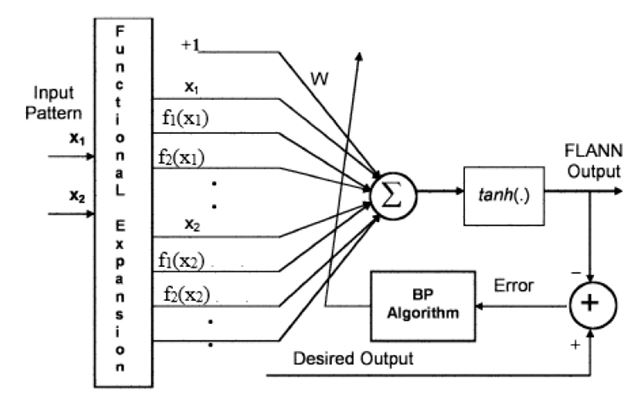
\includegraphics[width=1\textwidth,height=\textheight]{images/flann.jpg}
\caption{Functional Link Neural Network \label{fig:flann}}
\end{figure}

Figure \ref{fig:flann} shows each of the two inputs being expanded by the means of functions \(f_i\) where \(i \in [0,1, \ldots k-1]\). In the present study, the functions used are Chebyshev, Legendre, Power and Trigonometric as given in Equations \ref{eq:Chebyshev}, \ref{eq:Legendre}, \ref{eq:power} and \ref{eq:Trig} respectively

\begin{equation}
X_i=[1,x_i,( 2x_i^2-1),( 4x_i^3-3x_i ),( 8x_i^4-8x_i^2+1)] \label{eq:Chebyshev}
\end{equation}

\begin{equation}
X_i=[1,x_i,( 3x_i^2-1)/2,( 5x_i^3-3x_i)/2,( 35x_i^4-30x_i^2+3)/8] \label{eq:Legendre}
\end{equation}

\begin{equation}
X_i=[1,x_i,x_i^2,x_i^3,x_i^4]\label{eq:power}
\end{equation}

\begin{equation}
X_i=[x_i,\cos x_i, \sin x_i,\cos 2\pi x_i,\sin 2\pi x_i] \label{eq:Trig}
\end{equation}

The purpose of using FLANNs is to reduce training time and make the prediction more computationally efficient.

\hypertarget{complexity-comaprison-of-flann-and-mlp}{%
\subsection{Complexity Comaprison of FLANN and MLP}\label{complexity-comaprison-of-flann-and-mlp}}

The complexity of FLANN is lower than that of MLP. The greater the difference in network sizes of MLP and FLANN, the greater will be the reduction in complexity. The steps that each epoch will undergo in the training process are:

\begin{itemize}
\tightlist
\item
  Feedforward calculations to produce the output
\item
  Error Calculations for each layer
\item
  Modification of weights and biases during backpropagation
\end{itemize}

To mathematically compare the computational complexities of MLP and FLANN, consider a FLANN with architecture \({G-K}\) where G is the number of input variables to the neuron and K is the number of outputs (one in this study). For the same prediction problem, the corresponding MLP has an architecture \({H-I-K}\) where H is the reduced number of input variables prior to functional expansion, I is the number of neurons in the hidden layer and K is the same as described above i.e.~the number of outputs.

\begin{table}[t]

\caption{\label{tab:CompComplex}Computational Complexity}
\centering
\begin{tabular}{l|l|l}
\hline
\textbf{Operator} & \textbf{No. of Operations (MLP)} & \textbf{No. of Operations (FLANN)}\\
\hline
Addition & 2HI + 3IK + 3K & 2K(G+1) + K\\
\hline
Multiplication & 3HI + 4IK + 3I + 5K & 3K(G+1) + 2K\\
\hline
tanh(.) & I + K & K\\
\hline
\end{tabular}
\end{table}

The comparison has been shown in Table \ref{tab:CompComplex}

\clearpage

\hypertarget{results-and-analysis}{%
\section{Results and Analysis}\label{results-and-analysis}}

\hypertarget{trasmittance-experiment-1.1}{%
\subsection{Trasmittance Experiment 1.1}\label{trasmittance-experiment-1.1}}

This experiment involved training the neural network with just the wavelengths and predicting the transmittance (\%). The initial training was done on data corresponding to PFI concentration equal to 13.4. This training results were used to find the best architecture in terms if lowest Mean Squared Error (MSE), highest R squared and lowest training times. Since choosing an architecture by training the network just once isn't reliable, the training was done repeatedly 100 times. The MSEs, R squared values and the training times were then averaged over 100 ensembles. The results are recorded in Table \ref{tab:tableT1Nh}.

\begin{table}[t]

\caption{\label{tab:tableT1Nh}Performance of MLP with varying number of neurons}
\centering
\resizebox{\linewidth}{!}{
\fontsize{10}{12}\selectfont
\begin{tabular}{r|r|r|r|r|r}
\hline
Nh & Overall MSE (dB) & Test MSE (dB) & Train MSE (dB) & Avg. R Squared & Avg. Train Time (seconds)\\
\hline
3 & -15.87 & -13.70 & -17.24 & 0.980 & 1.81\\
\hline
4 & -16.18 & -13.74 & -17.84 & 0.983 & 1.82\\
\hline
5 & -16.15 & -13.61 & -17.90 & 0.983 & 1.81\\
\hline
6 & -16.18 & -13.61 & -17.98 & 0.983 & 2.02\\
\hline
7 & -16.05 & -13.54 & -17.79 & 0.983 & 2.02\\
\hline
\rowcolor{red}  \textcolor{white}{\textbf{8}} & \textcolor{white}{\textbf{-15.77}} & \textcolor{white}{\textbf{-13.04}} & \textcolor{white}{\textbf{-17.76}} & \textcolor{white}{\textbf{0.983}} & \textcolor{white}{\textbf{1.88}}\\
\hline
9 & -15.82 & -13.19 & -17.69 & 0.982 & 2.27\\
\hline
10 & -15.75 & -13.05 & -17.70 & 0.982 & 2.34\\
\hline
11 & -15.72 & -13.03 & -17.65 & 0.982 & 2.36\\
\hline
12 & -16.13 & -13.32 & -18.22 & 0.984 & 2.22\\
\hline
13 & -16.15 & -13.35 & -18.23 & 0.984 & 1.92\\
\hline
14 & -16.20 & -13.40 & -18.28 & 0.985 & 2.05\\
\hline
15 & -16.16 & -13.35 & -18.26 & 0.985 & 1.93\\
\hline
\end{tabular}}
\end{table}

As can be seen, 8 neurons is an appropriate choice, given that it gives appreciably low MSEs in a comparatively low training time. Using the \({1-8-1}\) architecture, its performance for concentration 13.4 in shown in Figure \ref{fig:transmitplot134}.

\begin{figure}
\centering
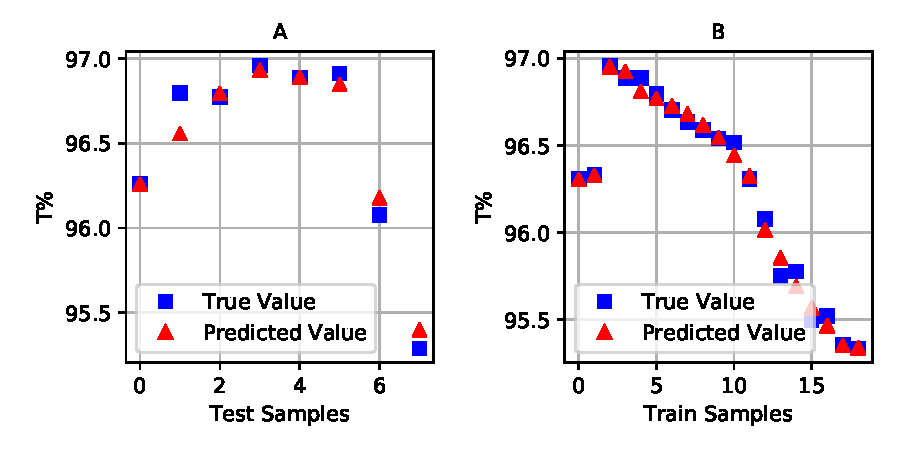
\includegraphics{Report_files/figure-latex/transmitplot134-1.pdf}
\caption{\label{fig:transmitplot134}\textbf{MLP results}: MLP Perfromance for PFI concentration 13.4 (A) Testing Dataset, and (B) Training Dataset}
\end{figure}

The performances on other concentrations are plotted in Figures \ref{fig:transmitplot0}, \ref{fig:transmitplot1}, \ref{fig:transmitplot25}, \ref{fig:transmitplot6} and \ref{fig:transmitplot30} for PFI concentrations 0, 1, 2.5, 6 and 30 respectively. This gives an idea for the overall performance of the network for any given concentration.

\begin{figure}
\centering
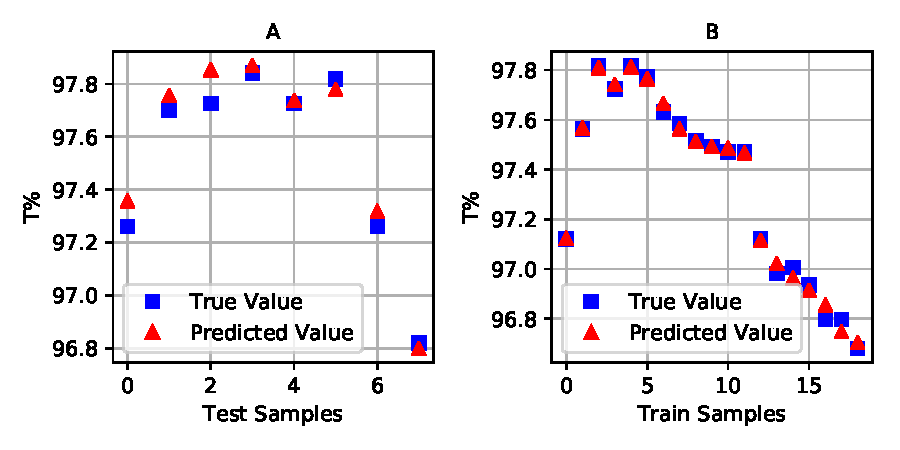
\includegraphics{Report_files/figure-latex/transmitplot0-1.pdf}
\caption{\label{fig:transmitplot0}\textbf{MLP results}: MLP Perfromance for PFI concentration 0 (A) Testing Dataset, and (B) Training Dataset}
\end{figure}

\begin{figure}
\centering
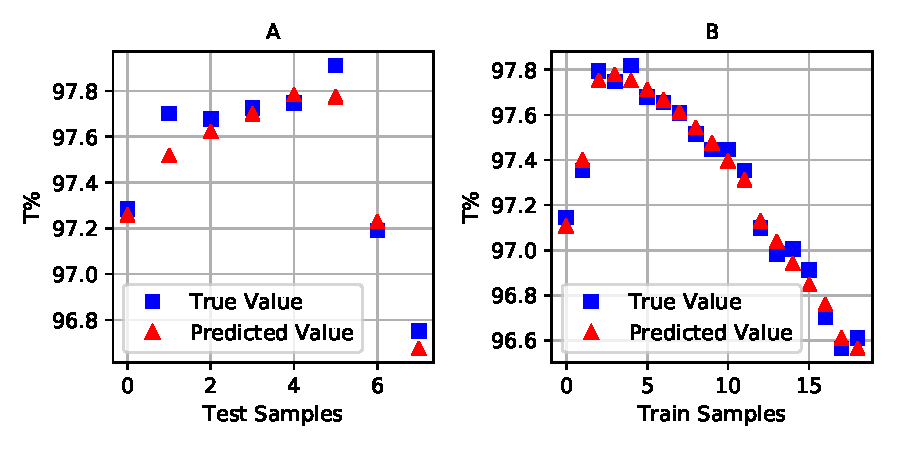
\includegraphics{Report_files/figure-latex/transmitplot1-1.pdf}
\caption{\label{fig:transmitplot1}\textbf{MLP results}: MLP Perfromance for PFI concentration 1.0 (A) Testing Dataset, and (B) Training Dataset}
\end{figure}

\begin{figure}
\centering
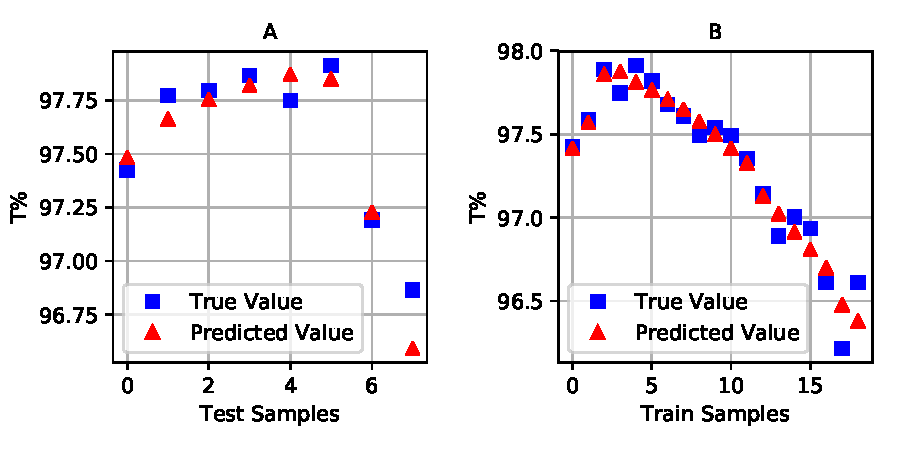
\includegraphics{Report_files/figure-latex/transmitplot25-1.pdf}
\caption{\label{fig:transmitplot25}\textbf{MLP results}: MLP Perfromance for PFI concentration 2.5 (A) Testing Dataset, and (B) Training Dataset}
\end{figure}

\begin{figure}
\centering
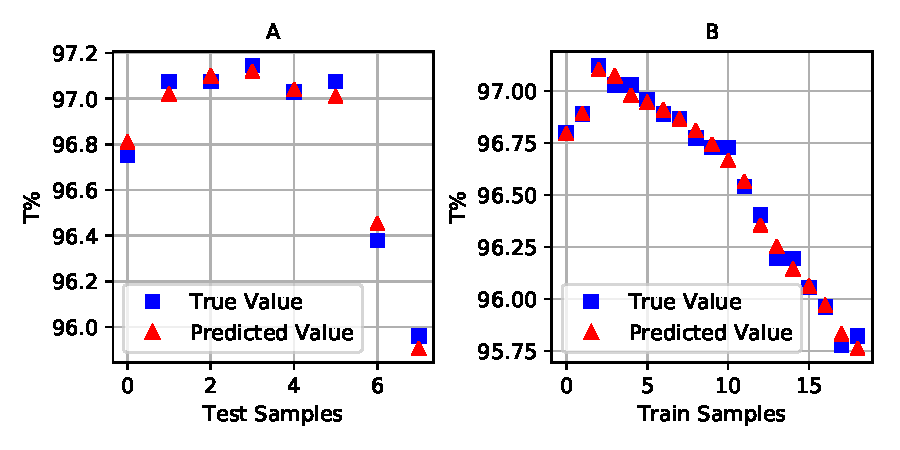
\includegraphics{Report_files/figure-latex/transmitplot6-1.pdf}
\caption{\label{fig:transmitplot6}\textbf{MLP results}: MLP Perfromance for PFI concentration 6 (A) Testing Dataset, and (B) Training Dataset}
\end{figure}

\begin{figure}
\centering
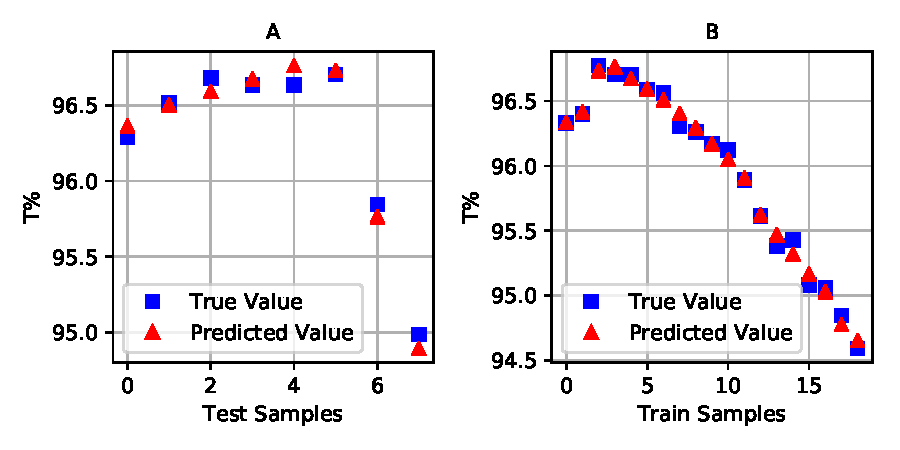
\includegraphics{Report_files/figure-latex/transmitplot30-1.pdf}
\caption{\label{fig:transmitplot30}\textbf{MLP results}: MLP Perfromance for PFI concentration 30 (A) Testing Dataset, and (B) Training Dataset}
\end{figure}

\newpage

\hypertarget{transmittance-experiment-1.2}{%
\subsection{Transmittance Experiment 1.2}\label{transmittance-experiment-1.2}}

The exact same experiment was repeated but this time using FLANN. The first step was to choose the better performing FLANN polynomial from among Chebyshev, Legendre, Power and Trigonometric, each having 5 polynomials. The bar charts given in Figure \ref{fig:transflannbar} show the performance of each FLANN polynomial in terms of average MSE and average training time over 100 ensembles. Chebyshev was chosen as it gave the most negative MSE in dB (lowest absolute value of MSE).

\begin{figure}
\centering
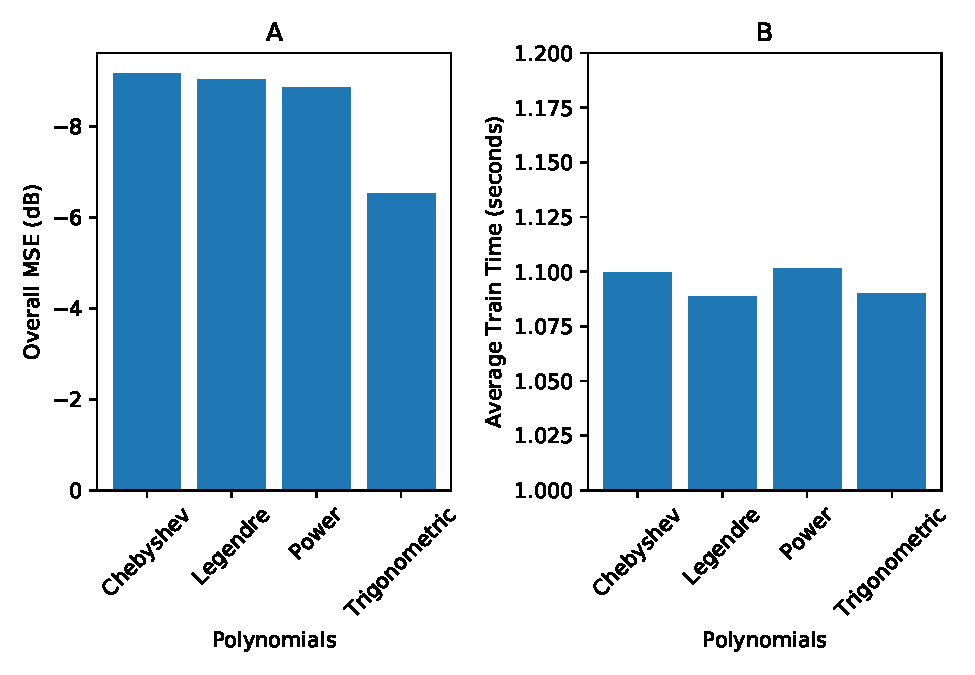
\includegraphics{Report_files/figure-latex/transflannbar-1.pdf}
\caption{\label{fig:transflannbar}\textbf{Choosing the best FLANN Polynomial}: Comparison Using (A) Resulting Mean Squared Error (MSE) and, (B) Average training time.}
\end{figure}

As in the case of MLP, the FLANN performance on PFI concentration 13.4, which is the concentration used to make the bar charts, is shown in \ref{fig:transmitflannplot134}.

\begin{figure}
\centering
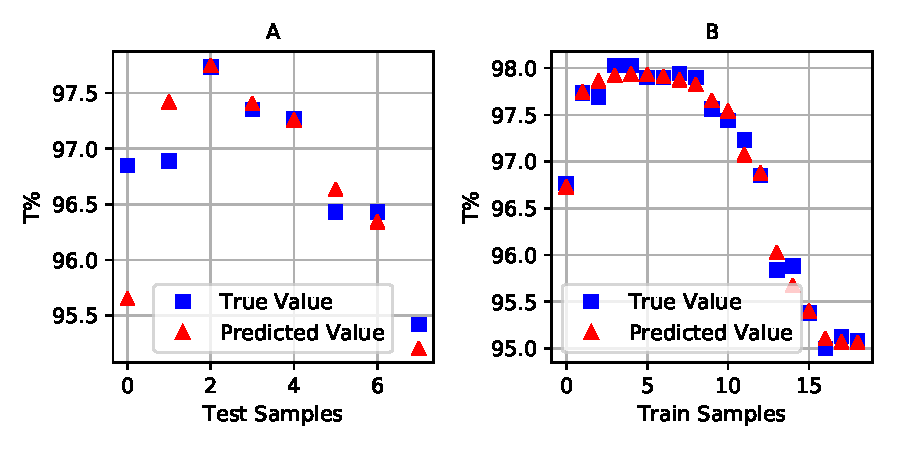
\includegraphics{Report_files/figure-latex/transmitflannplot134-1.pdf}
\caption{\label{fig:transmitflannplot134}\textbf{FLANN results}: FLANN Perfromance for PFI concentration 13.4 (A) Testing Dataset, and (B) Training Dataset}
\end{figure}

The performance on other concentrations are shown in Figures \ref{fig:transmitflannplot0}, \ref{fig:transmitflannplot1}, \ref{fig:transmitflannplot25}, \ref{fig:transmitflannplot6} and \ref{fig:transmitflannplot30} for concentration 0, 1, 2.5, 6 and 30 respectively.

\begin{figure}
\centering
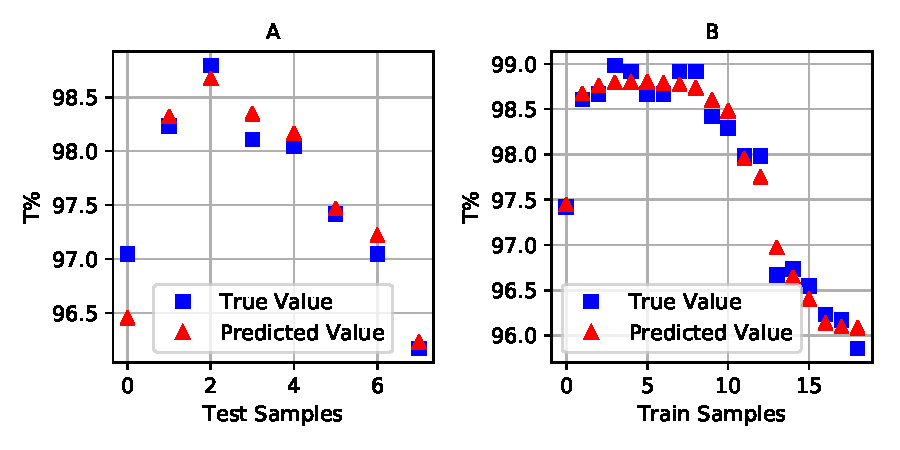
\includegraphics{Report_files/figure-latex/transmitflannplot0-1.pdf}
\caption{\label{fig:transmitflannplot0}\textbf{FLANN results}: FLANN Perfromance for PFI concentration 0 (A) Testing Dataset, and (B) Training Dataset}
\end{figure}

\begin{figure}
\centering
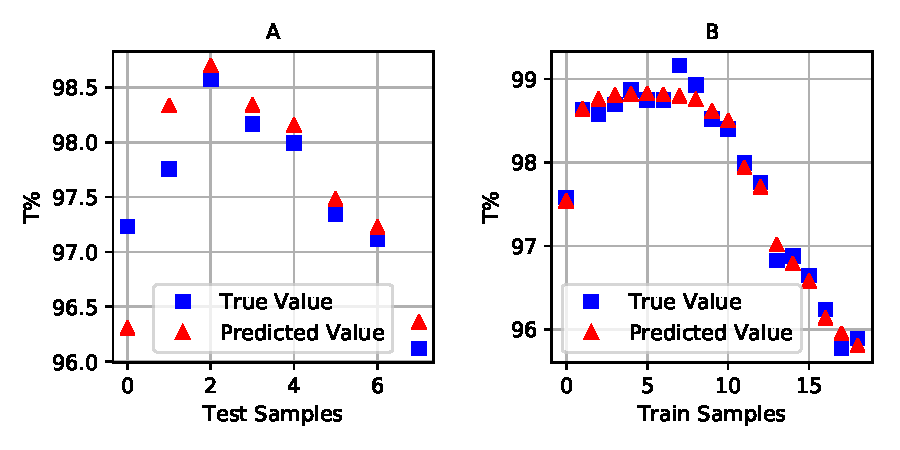
\includegraphics{Report_files/figure-latex/transmitflannplot1-1.pdf}
\caption{\label{fig:transmitflannplot1}\textbf{FLANN results}: FLANN Perfromance for PFI concentration 1 (A) Testing Dataset, and (B) Training Dataset}
\end{figure}

\begin{figure}
\centering
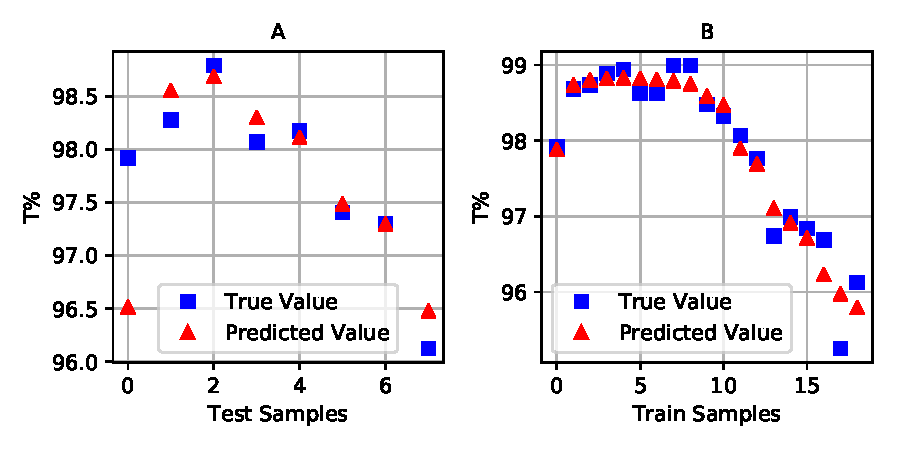
\includegraphics{Report_files/figure-latex/transmitflannplot25-1.pdf}
\caption{\label{fig:transmitflannplot25}\textbf{FLANN results}: FLANN Perfromance for PFI concentration 2.5 (A) Testing Dataset, and (B) Training Dataset}
\end{figure}

\begin{figure}
\centering
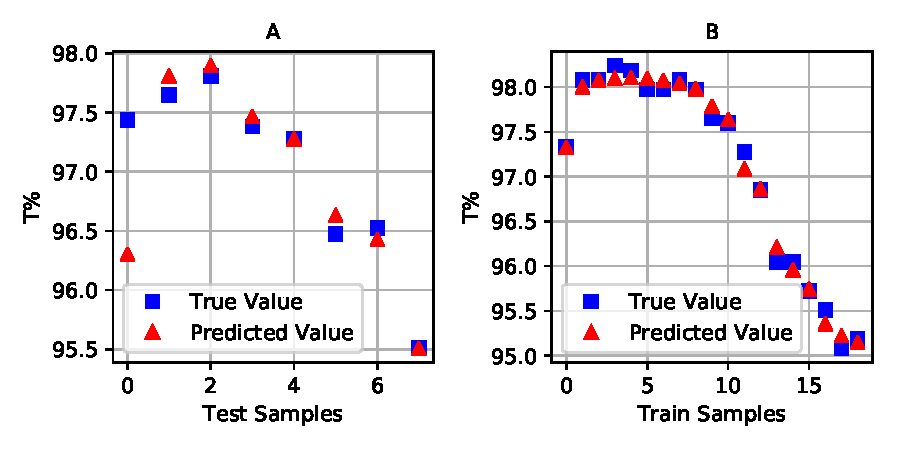
\includegraphics{Report_files/figure-latex/transmitflannplot6-1.pdf}
\caption{\label{fig:transmitflannplot6}\textbf{FLANN results}: FLANN Perfromance for PFI concentration 6 (A) Testing Dataset, and (B) Training Dataset}
\end{figure}

\begin{figure}
\centering
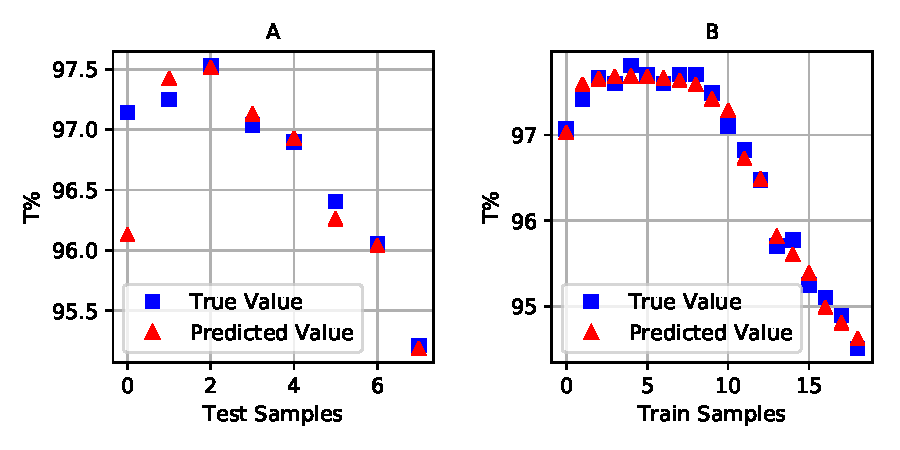
\includegraphics{Report_files/figure-latex/transmitflannplot30-1.pdf}
\caption{\label{fig:transmitflannplot30}\textbf{FLANN results}: FLANN Perfromance for PFI concentration 30 (A) Testing Dataset, and (B) Training Dataset}
\end{figure}

\newpage

\hypertarget{transmittance-experiment-1.3}{%
\subsection{Transmittance Experiment 1.3}\label{transmittance-experiment-1.3}}

The second part of the experiment with transmittance had two inputs to the ANN i.e.~wavelength and the concentration. That means that the ANN will be trained to predict the Transmittance (\%) of PEDOT:PSS layer given the wavelength and PFI concentration present. For this, different architectures were compared to arrive at the better performing one. The hidden layer was limited to one and the numbers of neurons were varied within it. The performance of each architecture is shown in Table \ref{tab:tableT2Nh}. The architecture with 12 neurons was chosen as it gave the lowest MSE, with similar training times as other architectures.

\begin{table}[t]

\caption{\label{tab:tableT2Nh}Performance of MLP with varying number of neurons}
\centering
\resizebox{\linewidth}{!}{
\fontsize{10}{12}\selectfont
\begin{tabular}{r|r|r|r|r|r}
\hline
Nh & Overall MSE (dB) & Test MSE (dB) & Train MSE (dB) & Avg. R Squared & Avg. Train Time (seconds)\\
\hline
3 & -13.50 & -13.08 & -13.70 & 0.957 & 1.17\\
\hline
4 & -17.42 & -16.73 & -17.76 & 0.983 & 1.16\\
\hline
5 & -17.56 & -16.71 & -17.98 & 0.984 & 1.17\\
\hline
6 & -18.50 & -17.33 & -19.12 & 0.988 & 1.18\\
\hline
7 & -18.62 & -17.61 & -19.13 & 0.988 & 1.23\\
\hline
8 & -18.37 & -17.14 & -19.03 & 0.987 & 1.33\\
\hline
9 & -18.95 & -17.79 & -19.57 & 0.989 & 1.34\\
\hline
10 & -18.72 & -17.52 & -19.37 & 0.988 & 1.23\\
\hline
11 & -18.95 & -17.80 & -19.57 & 0.989 & 1.23\\
\hline
\rowcolor{red}  \textcolor{white}{\textbf{12}} & \textcolor{white}{\textbf{-19.07}} & \textcolor{white}{\textbf{-17.91}} & \textcolor{white}{\textbf{-19.69}} & \textcolor{white}{\textbf{0.989}} & \textcolor{white}{\textbf{1.27}}\\
\hline
13 & -18.94 & -17.79 & -19.54 & 0.989 & 1.33\\
\hline
14 & -18.76 & -17.69 & -19.32 & 0.988 & 1.34\\
\hline
15 & -18.82 & -17.66 & -19.43 & 0.988 & 1.35\\
\hline
16 & -19.10 & -17.91 & -19.74 & 0.989 & 1.35\\
\hline
17 & -19.04 & -17.92 & -19.63 & 0.989 & 1.37\\
\hline
18 & -19.01 & -17.82 & -19.65 & 0.989 & 1.36\\
\hline
19 & -18.79 & -17.68 & -19.38 & 0.988 & 1.30\\
\hline
\end{tabular}}
\end{table}

Using the \{\(2-12-1\)\} architecture, the performance of the MLP is shown in \ref{fig:transmitplot2} for both the test and training samples. As obvious, the performance can be seen to be better on training samples compared to the testing samples as the MLP is familiar with the training dataset examples and has used them to train itself, while the testing dataset examples are new to the network.

\begin{figure}
\centering
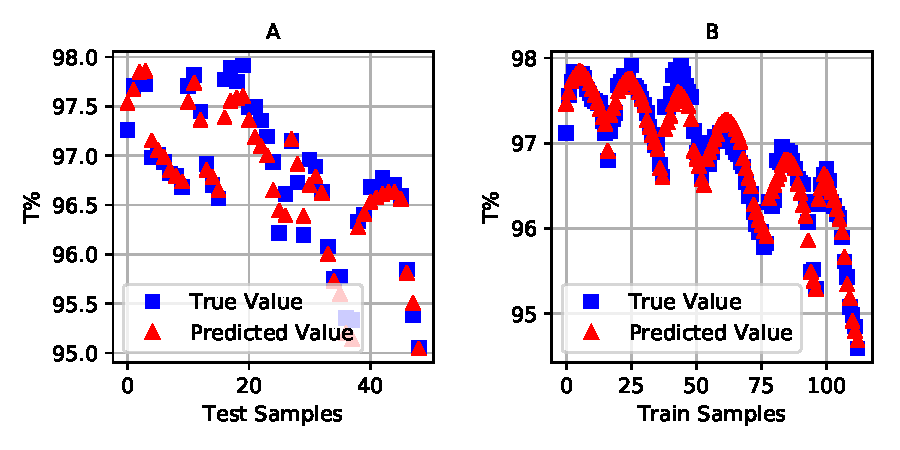
\includegraphics{Report_files/figure-latex/transmitplot2-1.pdf}
\caption{\label{fig:transmitplot2}\textbf{MLP results}: MLP Perfromance on (A) Testing Dataset, and (B) Training Dataset}
\end{figure}

One possible application for such a network can be to predict the transmittance of the PEDOT:PSS layer with a specific PFI concentration prior to manufacturing the layer. The optical characteristics, if known beforehand, can assist in assessing the usefulness of the PEDOT:PSS layer in the practical applications at hand. With this in mind, the MLP was provided a new unknown concentration and wavelength values in the range given in Figure \ref{fig:transfig}. The two PFI concentrations of 29 and 15 were chosen because of their numerical closeness to the already known concentrations of 30 and 13.4 respectively. This allowed the plotting of transmittance vs.~wavelength characteristics of both concentrations, one new (i.e.~29 or 15) and one already known (30 or 13.4) on the same figure. Ideally, their lines should follow close to each other because both concentrations are almost equal. The results are given in Figure \ref{fig:transnew}. As can be seen, the predictions seem pretty accurate as the two lines are very close to each other.

\begin{figure}
\centering
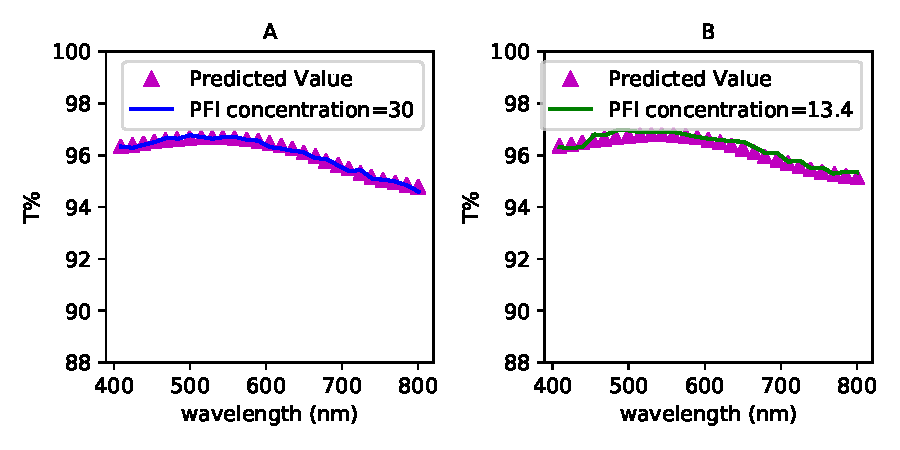
\includegraphics{Report_files/figure-latex/transnew-1.pdf}
\caption{\label{fig:transnew}\textbf{Predicting Transmittance of a new PFI concentration }: (A) A new PFI concentration of 29, (B) A new PFI concentration of 15.}
\end{figure}

\newpage

\hypertarget{transmittance-experiment-1.4}{%
\subsection{Transmittance Experiment 1.4}\label{transmittance-experiment-1.4}}

Based on the bar chart of Figure \ref{fig:transflannbar2}, Trigonometric FLANN has the lowest MSE. Therefore, we have chosen Trigonometric FLANN. Its performance on the dataset can be seen in Figure \ref{fig:transmitflannplot2}.


\begin{figure}
\centering
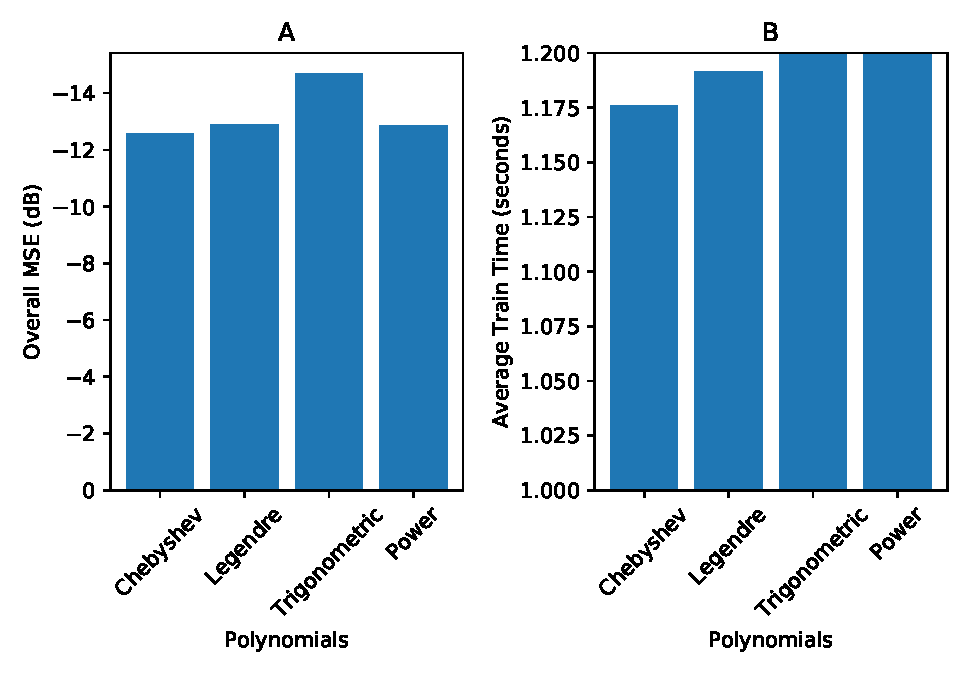
\includegraphics{Report_files/figure-latex/transflannbar2-1.pdf}
\caption{\label{fig:transflannbar2}\textbf{Choosing the best FLANN Polynomial}: Comparison Using (A) Resulting Mean Squared Error (MSE) and, (B) Average training time.}
\end{figure}

\begin{figure}
\centering
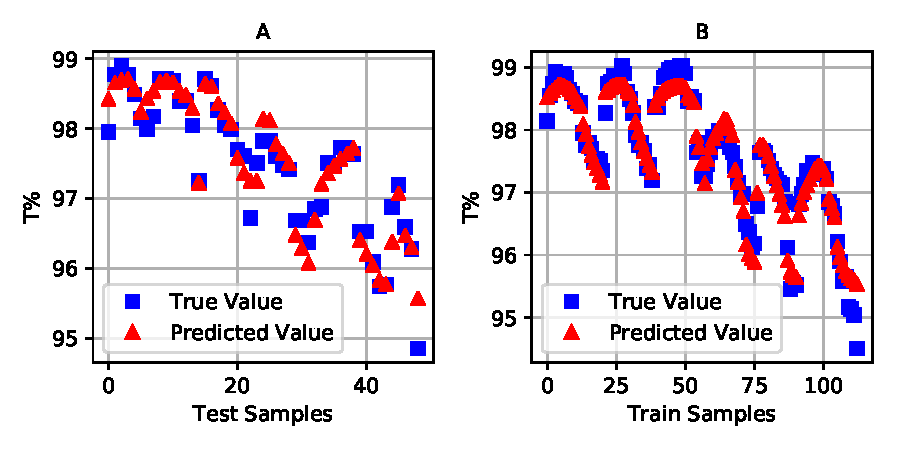
\includegraphics{Report_files/figure-latex/transmitflannplot2-1.pdf}
\caption{\label{fig:transmitflannplot2}\textbf{FLANN results}: FLANN Perfromance for (A) Testing Dataset, and (B) Training Dataset}
\end{figure}

The transmittance percentage of new PFI concentrations 29 and 15 are shown in\ref{fig:transflannnew}. The performance of FLANN isn't as good as it was of the MLP. Notice how the predicted values fluctuate above and below the already known transmittance values of almost equal concentrations. For this purpose, MLP will be chosen as it gave a better, more reliable performance.

\begin{figure}
\centering
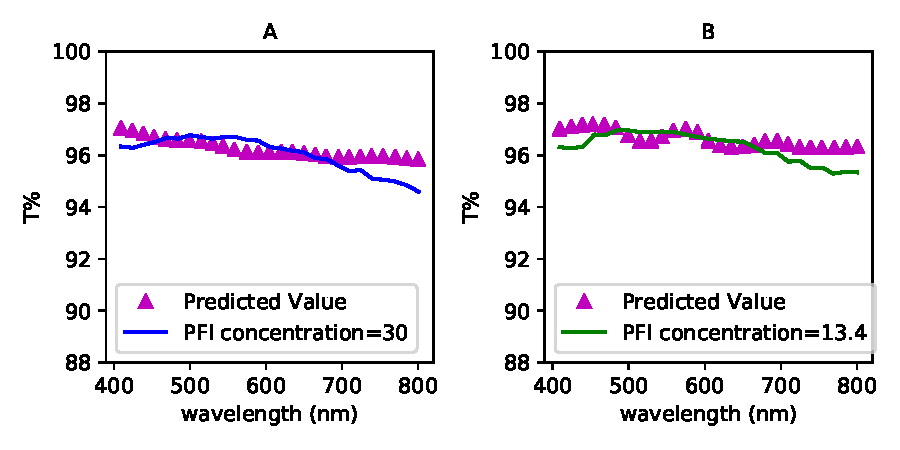
\includegraphics{Report_files/figure-latex/transflannnew-1.pdf}
\caption{\label{fig:transflannnew}\textbf{Predicting Transmittance of a new PFI concentration }: (A) A new PFI concentration of 29, (B) A new PFI concentration of 15.}
\end{figure}

\newpage

\hypertarget{current-density-experiment-2.1}{%
\subsection{Current Density Experiment 2.1}\label{current-density-experiment-2.1}}

Experiments similar to the transmittance vs.~wavelength characteristic were conducted for the current density vs.~voltage characteristic as well. That means the first experiment involved predicting, for any one PFI concentration, the current density when voltage is provided as an input to the ANN. Just as before, the PFI concentration chosen was 13.4 in order to select the best performing architecture. The numbers of neurons in the hidden layer were varied and their effect on averages of MSE, R squared and training times over 100 ensembles were recorded in Table \ref{tab:tableJV1Nh}. The architecture \({1-8-1}\) gave high enough average MSEs for overall, training and test dataset with appreciable training times.

\begin{table}[t]

\caption{\label{tab:tableJV1Nh}Performance of MLP with varying number of neurons}
\centering
\resizebox{\linewidth}{!}{
\fontsize{10}{12}\selectfont
\begin{tabular}{r|r|r|r|r|r}
\hline
Nh & Overall MSE (dB) & Test MSE (dB) & Train MSE (dB) & Avg. R Squared & Avg. Train Time\\
\hline
3 & -22.27 & -18.96 & -24.82 & 0.997 & 1.05\\
\hline
4 & -22.54 & -19.26 & -25.04 & 0.997 & 1.01\\
\hline
5 & -22.96 & -19.45 & -25.84 & 0.997 & 1.04\\
\hline
6 & -22.85 & -19.35 & -25.72 & 0.997 & 1.13\\
\hline
7 & -23.04 & -19.50 & -25.96 & 0.997 & 1.14\\
\hline
\rowcolor{red}  \textcolor{white}{\textbf{8}} & \textcolor{white}{\textbf{-23.02}} & \textcolor{white}{\textbf{-19.46}} & \textcolor{white}{\textbf{-25.98}} & \textcolor{white}{\textbf{0.997}} & \textcolor{white}{\textbf{1.13}}\\
\hline
9 & -23.26 & -19.58 & -26.43 & 0.998 & 1.13\\
\hline
10 & -23.13 & -19.50 & -26.21 & 0.998 & 1.23\\
\hline
11 & -23.02 & -19.43 & -26.04 & 0.997 & 1.14\\
\hline
12 & -23.05 & -19.51 & -25.98 & 0.997 & 1.16\\
\hline
13 & -22.91 & -19.34 & -25.90 & 0.997 & 1.17\\
\hline
14 & -22.95 & -19.38 & -25.93 & 0.997 & 1.16\\
\hline
15 & -22.95 & -19.41 & -25.88 & 0.997 & 1.18\\
\hline
16 & -23.00 & -19.43 & -25.96 & 0.997 & 1.19\\
\hline
17 & -22.99 & -19.44 & -25.93 & 0.997 & 1.12\\
\hline
18 & -23.00 & -19.46 & -25.92 & 0.997 & 1.09\\
\hline
19 & -23.20 & -19.59 & -26.24 & 0.997 & 1.10\\
\hline
\end{tabular}}
\end{table}

The actual vs.~predicted values for concentration 13.4 are shown in \ref{fig:JVplot134}.

\begin{figure}
\centering
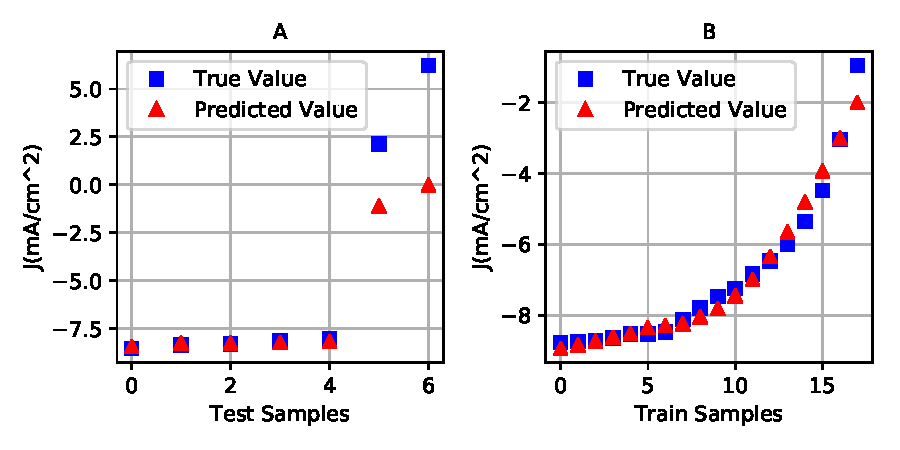
\includegraphics{Report_files/figure-latex/JVplot134-1.pdf}
\caption{\label{fig:JVplot134}\textbf{MLP results}: MLP Perfromance for PFI concentration 13.4 (A) Testing Dataset, and (B) Training Dataset}
\end{figure}

The performance of the chosen MLP for PFI concentrations 0, 1 and 30 are shown in \ref{fig:JVplot0}, \ref{fig:JVplot1} and \ref{fig:JVplot30} respectively.

\begin{figure}
\centering
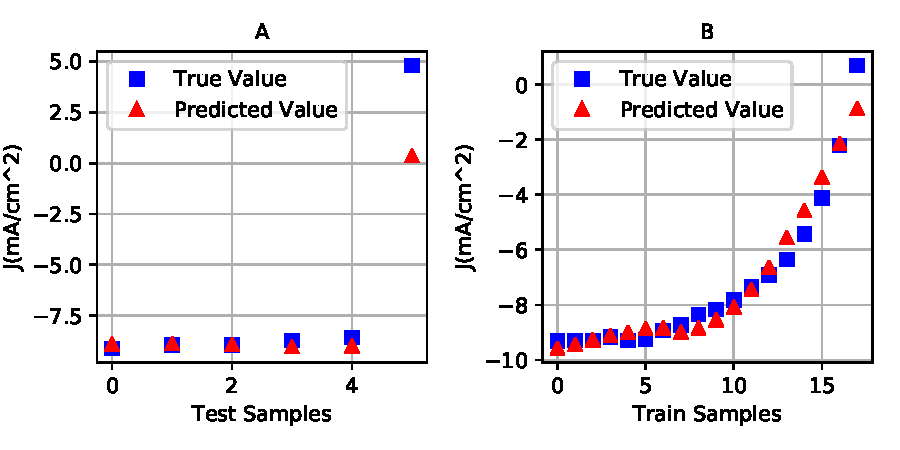
\includegraphics{Report_files/figure-latex/JVplot0-1.pdf}
\caption{\label{fig:JVplot0}\textbf{MLP results}: MLP Perfromance for PFI concentration 0 (A) Testing Dataset, and (B) Training Dataset}
\end{figure}

\begin{figure}
\centering
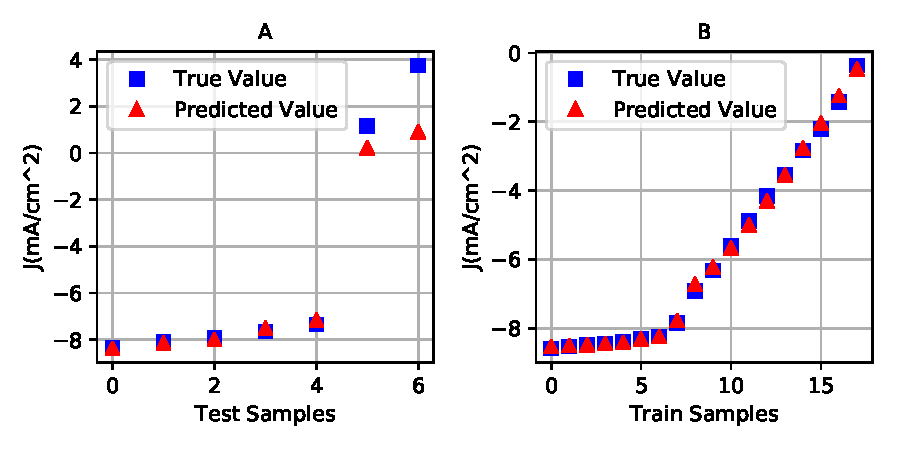
\includegraphics{Report_files/figure-latex/JVplot1-1.pdf}
\caption{\label{fig:JVplot1}\textbf{MLP results}: MLP Perfromance for PFI concentration 1 (A) Testing Dataset, and (B) Training Dataset}
\end{figure}

\begin{figure}
\centering
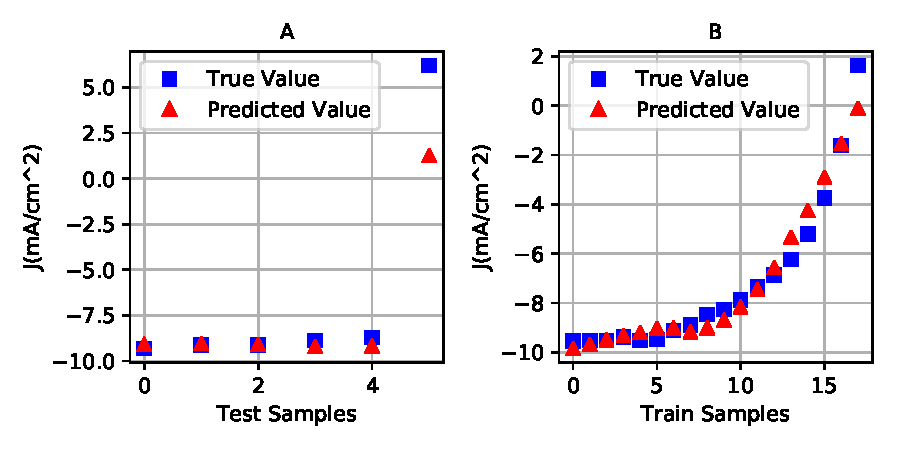
\includegraphics{Report_files/figure-latex/JVplot30-1.pdf}
\caption{\label{fig:JVplot30}\textbf{MLP results}: MLP Perfromance for PFI concentration 30 (A) Testing Dataset, and (B) Training Dataset}
\end{figure}

\newpage

\hypertarget{current-density-experiment-2.2}{%
\subsection{Current Density Experiment 2.2}\label{current-density-experiment-2.2}}

For the same problem, a FLANN was used instead of MLP. The different polynomials were tested for their suitability and the results are shown in Figure \ref{fig:jvflannbar}. As in the case of transmittance for the corresponding experiment, the preferred polynomial is Chebyshev due to its most negative average MSE and lowest average training time.

\begin{figure}
\centering
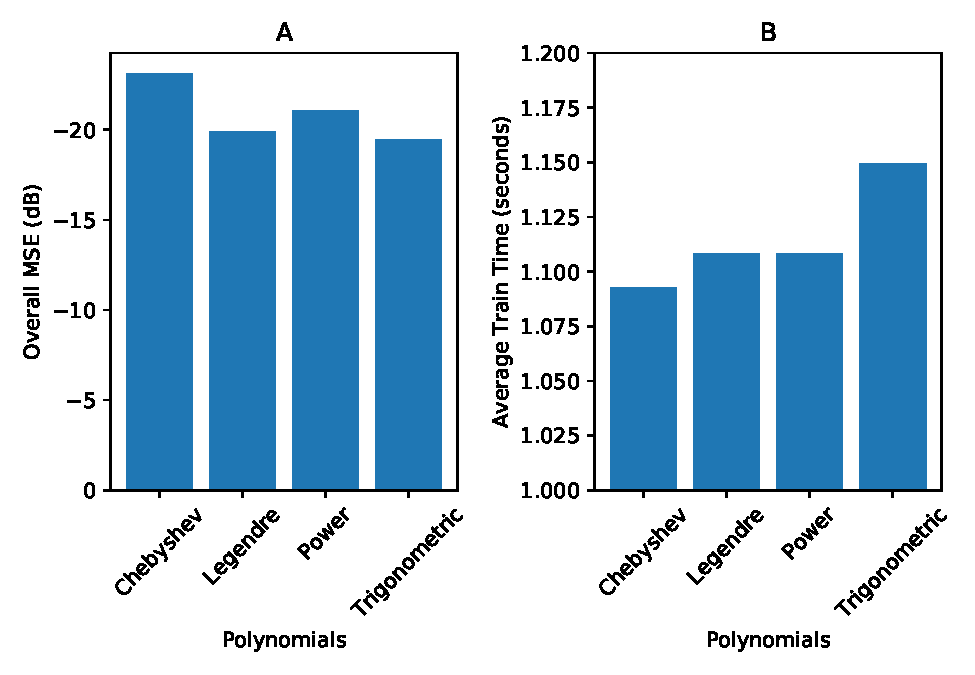
\includegraphics{Report_files/figure-latex/jvflannbar-1.pdf}
\caption{\label{fig:jvflannbar}\textbf{Choosing the best FLANN Polynomial}: Comparison Using (A) Resulting Mean Squared Error (MSE) and, (B) Average training time.}
\end{figure}

Its performance for PFI concentration 13.4 is shown in Figure \ref{fig:JVflannplot134}.

\begin{figure}
\centering
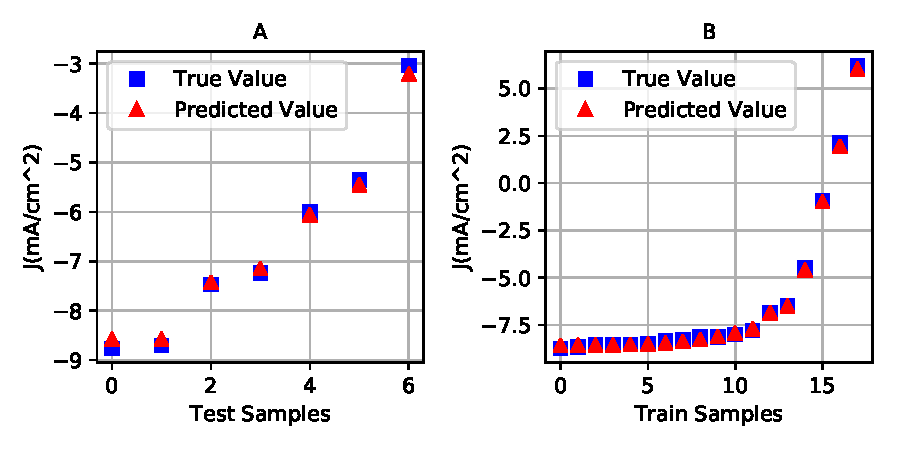
\includegraphics{Report_files/figure-latex/JVflannplot134-1.pdf}
\caption{\label{fig:JVflannplot134}\textbf{FLANN results}: FLANN Perfromance for PFI concentration 13.4 (A) Testing Dataset, and (B) Training Dataset}
\end{figure}

Performance of Chebyshev FLANN on PFI concentrations 0, 1 and 30 are shown in Figures \ref{fig:JVflannplot0}, \ref{fig:JVflannplot1} and \ref{fig:JVflannplot30} respectively.

\begin{figure}
\centering
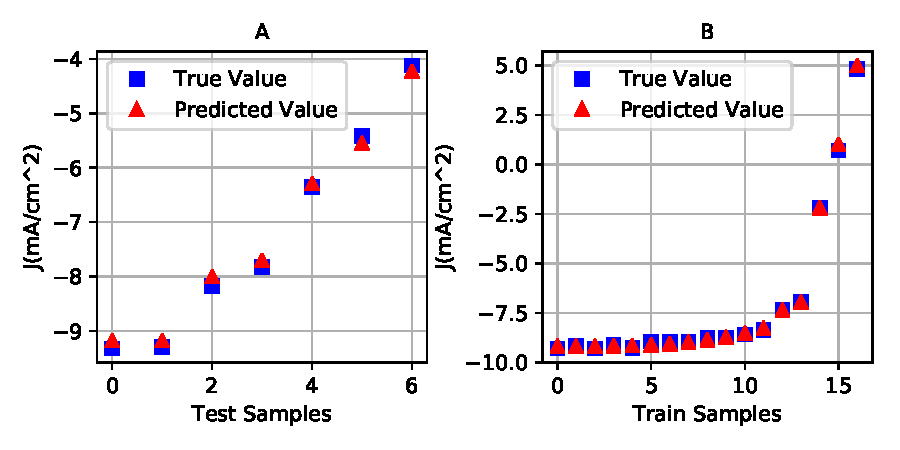
\includegraphics{Report_files/figure-latex/JVflannplot0-1.pdf}
\caption{\label{fig:JVflannplot0}\textbf{FLANN results}: FLANN Perfromance for PFI concentration 0 (A) Testing Dataset, and (B) Training Dataset}
\end{figure}

\begin{figure}
\centering
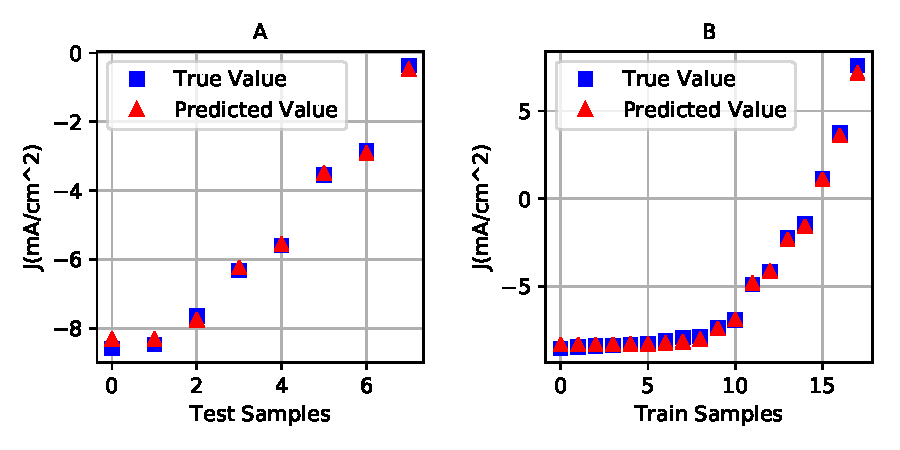
\includegraphics{Report_files/figure-latex/JVflannplot1-1.pdf}
\caption{\label{fig:JVflannplot1}\textbf{FLANN results}: FLANN Perfromance for PFI concentration 1 (A) Testing Dataset, and (B) Training Dataset}
\end{figure}

\begin{figure}
\centering
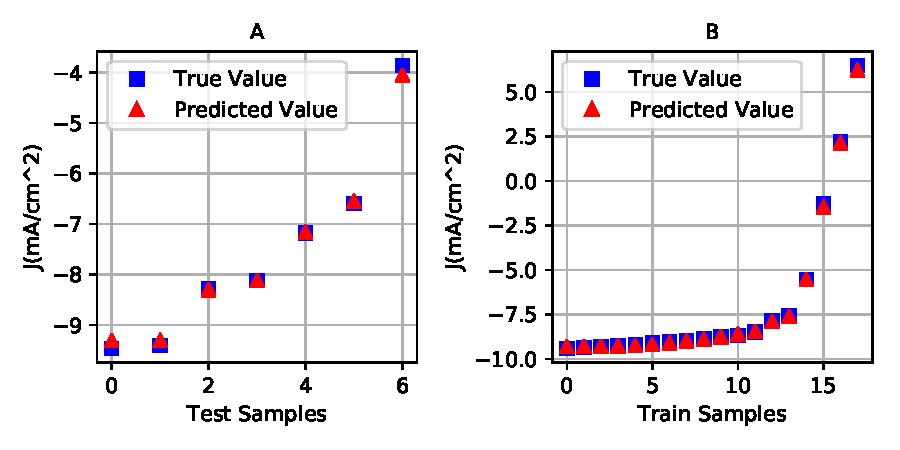
\includegraphics{Report_files/figure-latex/JVflannplot30-1.pdf}
\caption{\label{fig:JVflannplot30}\textbf{FLANN results}: FLANN Perfromance for PFI concentration 30 (A) Testing Dataset, and (B) Training Dataset}
\end{figure}

\newpage

\hypertarget{current-density-experiment-2.3}{%
\subsection{Current Density Experiment 2.3}\label{current-density-experiment-2.3}}

The second experiment on current density vs.~voltage involved predicting current density based on voltage and PFI concentration present in the HEL layer. The ANN therefore had two input neurons and the neurons in the hidden layer were varied as given in Table \ref{tab:tableJV2Nh}. The architecture \({2-12-1}\) was chosen due to its low average MSEs and high average R squared values.

\begin{table}[t]

\caption{\label{tab:tableJV2Nh}Performance of MLP with varying number of neurons}
\centering
\resizebox{\linewidth}{!}{
\fontsize{10}{12}\selectfont
\begin{tabular}{r|r|r|r|r|r}
\hline
Nh & Overall MSE (dB) & Test MSE (dB) & Train MSE (dB) & Avg. R Squared & Avg. Train Time\\
\hline
3 & -14.76 & -13.84 & -15.22 & 0.969 & 1.31\\
\hline
4 & -15.11 & -14.17 & -15.59 & 0.972 & 1.31\\
\hline
5 & -16.08 & -14.42 & -17.04 & 0.980 & 1.36\\
\hline
6 & -16.94 & -15.46 & -17.77 & 0.983 & 1.31\\
\hline
7 & -16.87 & -15.49 & -17.64 & 0.982 & 1.33\\
\hline
8 & -19.67 & -18.36 & -20.38 & 0.991 & 1.32\\
\hline
9 & -16.72 & -15.41 & -17.43 & 0.981 & 1.34\\
\hline
10 & -16.57 & -15.36 & -17.20 & 0.980 & 1.34\\
\hline
11 & -17.79 & -16.47 & -18.51 & 0.985 & 1.34\\
\hline
\rowcolor{red}  \textcolor{white}{\textbf{12}} & \textcolor{white}{\textbf{-19.31}} & \textcolor{white}{\textbf{-17.93}} & \textcolor{white}{\textbf{-20.07}} & \textcolor{white}{\textbf{0.990}} & \textcolor{white}{\textbf{1.36}}\\
\hline
13 & -17.35 & -15.82 & -18.21 & 0.984 & 1.35\\
\hline
14 & -16.84 & -15.40 & -17.64 & 0.982 & 1.36\\
\hline
15 & -16.67 & -15.30 & -17.42 & 0.981 & 1.36\\
\hline
16 & -19.41 & -18.06 & -20.14 & 0.990 & 1.37\\
\hline
17 & -16.84 & -15.62 & -17.49 & 0.981 & 1.40\\
\hline
18 & -16.94 & -15.58 & -17.68 & 0.982 & 1.38\\
\hline
19 & -19.18 & -17.76 & -19.97 & 0.990 & 1.40\\
\hline
\end{tabular}}
\end{table}

The performance of the MLP is shown in Figure \ref{fig:JVplot2}

\begin{figure}
\centering
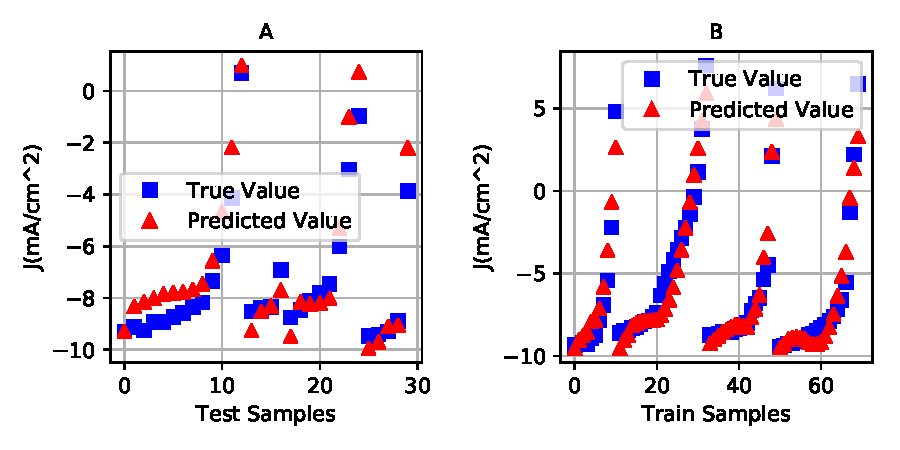
\includegraphics{Report_files/figure-latex/JVplot2-1.pdf}
\caption{\label{fig:JVplot2}\textbf{MLP results}: MLP Perfromance on (A) Testing Dataset, and (B) Training Dataset}
\end{figure}

The MLP will be used for prediction for a new concentration for which we don't have the experimental data. The new PFI concentrations are 29 and 15 and the predicted values are shown against another numerically close, known concentration in Figure \ref{fig:JVnew}

\begin{figure}
\centering
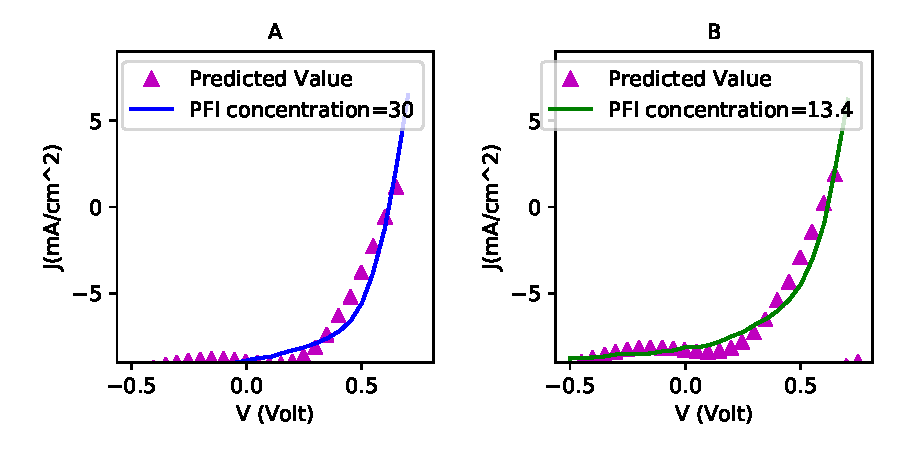
\includegraphics{Report_files/figure-latex/JVnew-1.pdf}
\caption{\label{fig:JVnew}\textbf{Predicting Transmittance of a new PFI concentration }: (A) A new PFI concentration of 29, (B) A new PFI concentration of 15.}
\end{figure}

\newpage

\hypertarget{current-density-experiment-2.4}{%
\subsection{Current Density Experiment 2.4}\label{current-density-experiment-2.4}}

As can be seen in \ref{fig:jvflannbar2}, the Power polynomial gives good results in terms of both average MSE and average training time. Its performance is shown in Figure \ref{fig:jvflannplot2} for both test and training data.

\begin{figure}
\centering
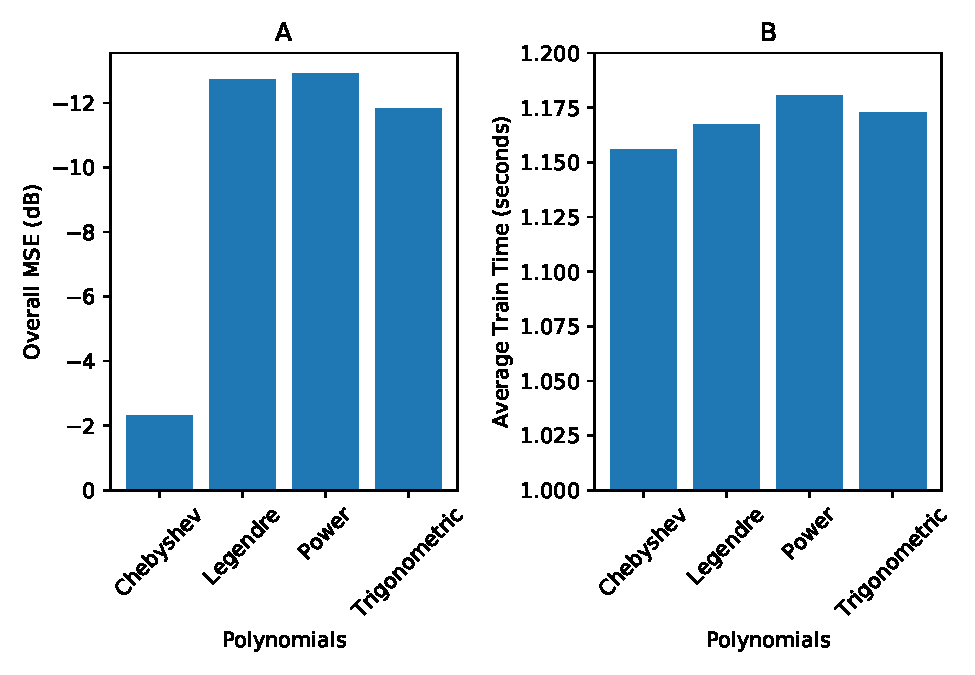
\includegraphics{Report_files/figure-latex/jvflannbar2-1.pdf}
\caption{\label{fig:jvflannbar2}\textbf{Choosing the best FLANN Polynomial}: Comparison Using (A) Resulting Mean Squared Error (MSE) and, (B) Average training time.}
\end{figure}

\begin{figure}
\centering
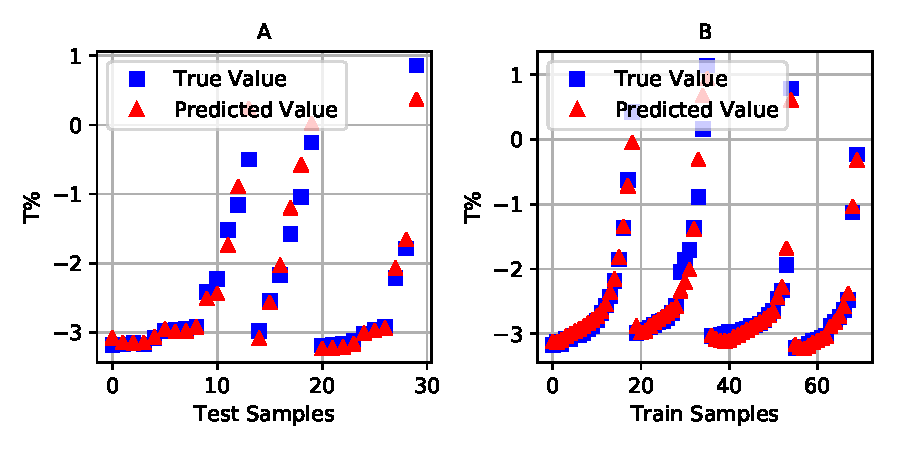
\includegraphics{Report_files/figure-latex/jvflannplot2-1.pdf}
\caption{\label{fig:jvflannplot2}\textbf{FLANN results}: FLANN Perfromance for (A) Testing Dataset, and (B) Training Dataset}
\end{figure}

As done previously, the new PFI concentrations chosen are 29 and 15 and their results are given in \ref{fig:jvflannnew}. The new concentrations follow closely with the known concentrations , thus indicating that FLANN is working properly.

\begin{figure}
\centering
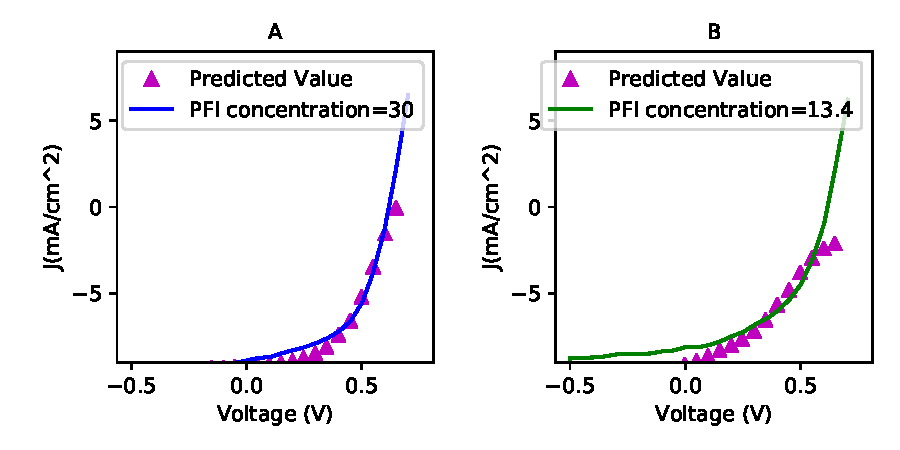
\includegraphics{Report_files/figure-latex/jvflannnew-1.pdf}
\caption{\label{fig:jvflannnew}\textbf{Predicting Current Density of a new PFI concentration }: (A) A new PFI concentration of 29, (B) A new PFI concentration of 15.}
\end{figure}

\hypertarget{conclusion}{%
\section{Conclusion}\label{conclusion}}

The modeling of transmittance vs.~wavelength and current density vs.~voltage for OPVs containing PFI additive in the PEDOT:PSS hole extracting layer can be done to a reasonable accuracy. Except for the single input ANN in the case of current density vs.~voltage characteristic, the accuracies obtained through MLP were always slightly higher than through FLANN. FLANN, however, had an edge in terms of having lower training times.

\newpage

\hypertarget{references}{%
\section{References}\label{references}}

\widowpenalty=150
\clubpenalty=150

\hypertarget{appendix-appendix}{%
\appendix}


\hypertarget{refs}{}
\leavevmode\hypertarget{ref-Hoth2008}{}%
{[}1{]} C. N. Hoth, P. Schilinsky, S. A. Choulis, and C. J. Brabec, ``Printing Highly Efficient Organic Solar Cells,'' \emph{Nano Letters}, vol. 8, no. 9, pp. 2806--2813, Sep. 2008.

\leavevmode\hypertarget{ref-Manceau2011}{}%
{[}2{]} M. Manceau, D. Angmo, M. Jørgensen, and F. C. Krebs, ``ITO-free flexible polymer solar cells: From small model devices to roll-to-roll processed large modules,'' \emph{Organic Electronics}, vol. 12, no. 4, pp. 566--574, Apr. 2011.

\leavevmode\hypertarget{ref-Krebs2009}{}%
{[}3{]} F. C. Krebs, ``Fabrication and processing of polymer solar cells: A review of printing and coating techniques,'' \emph{Solar Energy Materials and Solar Cells}, vol. 93, no. 4, pp. 394--412, Apr. 2009.

\leavevmode\hypertarget{ref-Ribierre2011}{}%
{[}4{]} J. Ribierre, T. Aoyama, T. Muto, and P. André, ``Hybrid organic--inorganic liquid bistable memory devices,'' \emph{Organic Electronics}, vol. 12, no. 11, pp. 1800--1805, Nov. 2011.

\leavevmode\hypertarget{ref-Kim2014}{}%
{[}5{]} R. H. Kim \emph{et al.}, ``Non-volatile organic memory with sub-millimetre bending radius,'' \emph{Nature Communications}, vol. 5, no. 1, p. 3583, May 2014.

\leavevmode\hypertarget{ref-Andersen2014}{}%
{[}6{]} T. R. Andersen \emph{et al.}, ``Scalable, ambient atmosphere roll-to-roll manufacture of encapsulated large area, flexible organic tandem solar cell modules,'' \emph{Energy \& Environmental Science}, vol. 7, no. 9, p. 2925, Jun. 2014.

\leavevmode\hypertarget{ref-Mazzio2015}{}%
{[}7{]} K. A. Mazzio and C. K. Luscombe, ``Correction: The future of organic photovoltaics,'' \emph{Chemical Society Reviews}, vol. 44, no. 15, pp. 5744--5744, Jul. 2015.

\leavevmode\hypertarget{ref-Ribierre2015}{}%
{[}8{]} J. C. Ribierre \emph{et al.}, ``Ambipolar organic field-effect transistors based on solution-processed single crystal microwires of a quinoidal oligothiophene derivative,'' \emph{Chem. Commun.}, vol. 51, no. 27, pp. 5836--5839, Mar. 2015.

\leavevmode\hypertarget{ref-Gu2017}{}%
{[}9{]} X. Gu \emph{et al.}, ``Roll-to-Roll Printed Large-Area All-Polymer Solar Cells with 5\% Efficiency Based on a Low Crystallinity Conjugated Polymer Blend,'' \emph{Advanced Energy Materials}, vol. 7, no. 14, p. 1602742, Jul. 2017.

\leavevmode\hypertarget{ref-Stevenson2015}{}%
{[}10{]} J. R. Y. Stevenson, S. Lattante, P. André, M. Anni, and G. A. Turnbull, ``Fabrication of free-standing ordered fluorescent polymer nanofibres by electrospinning,'' \emph{Applied Physics Letters}, vol. 106, no. 17, p. 173301, Apr. 2015.

\leavevmode\hypertarget{ref-Joly2016}{}%
{[}11{]} D. Joly, J.-W. Jung, I.-D. Kim, and R. Demadrille, ``Electrospun materials for solar energy conversion: innovations and trends,'' \emph{Journal of Materials Chemistry C}, vol. 4, no. 43, pp. 10173--10197, Nov. 2016.

\leavevmode\hypertarget{ref-Koppitz2017}{}%
{[}12{]} M. Koppitz \emph{et al.}, ``Organic Solar Modules: Fully Doctor Bladed on Glass in Air,'' \emph{Energy Technology}, vol. 5, no. 7, pp. 1105--1111, Jul. 2017.

\leavevmode\hypertarget{ref-You2013}{}%
{[}13{]} J. You \emph{et al.}, ``A polymer tandem solar cell with 10.6\% power conversion efficiency,'' \emph{Nature Communications}, vol. 4, no. 1, p. 1446, Jun. 2013.

\leavevmode\hypertarget{ref-Zhao2016}{}%
{[}14{]} W. Zhao \emph{et al.}, ``Fullerene-Free Polymer Solar Cells with over 11\% Efficiency and Excellent Thermal Stability,'' \emph{Advanced Materials}, vol. 28, no. 23, pp. 4734--4739, Jun. 2016.

\leavevmode\hypertarget{ref-Chen2015}{}%
{[}15{]} J.-D. Chen \emph{et al.}, ``Single-Junction Polymer Solar Cells Exceeding 10\% Power Conversion Efficiency,'' \emph{Advanced Materials}, vol. 27, no. 6, pp. 1035--1041, Feb. 2015.

\leavevmode\hypertarget{ref-Park2016}{}%
{[}16{]} K. H. Park, Y. An, S. Jung, H. Park, and C. Yang, ``The use of an n-type macromolecular additive as a simple yet effective tool for improving and stabilizing the performance of organic solar cells,'' \emph{Energy \& Environmental Science}, vol. 9, no. 11, pp. 3464--3471, Nov. 2016.

\leavevmode\hypertarget{ref-Scharber2006}{}%
{[}17{]} M. C. Scharber \emph{et al.}, ``Design Rules for Donors in Bulk-Heterojunction Solar Cells---Towards 10 \% Energy-Conversion Efficiency,'' \emph{Advanced Materials}, vol. 18, no. 6, pp. 789--794, Mar. 2006.

\leavevmode\hypertarget{ref-Brabec2002}{}%
{[}18{]} C. J. Brabec, S. E. Shaheen, C. Winder, N. S. Sariciftci, and P. Denk, ``Effect of LiF/metal electrodes on the performance of plastic solar cells,'' \emph{Applied Physics Letters}, vol. 80, no. 7, pp. 1288--1290, Feb. 2002.

\leavevmode\hypertarget{ref-Brown1999}{}%
{[}19{]} T. M. Brown, J. S. Kim, R. H. Friend, F. Cacialli, R. Daik, and W. J. Feast, ``Built-in field electroabsorption spectroscopy of polymer light-emitting diodes incorporating a doped poly(3,4-ethylene dioxythiophene) hole injection layer,'' \emph{Applied Physics Letters}, vol. 75, no. 12, pp. 1679--1681, Sep. 1999.

\leavevmode\hypertarget{ref-DeJong2000}{}%
{[}20{]} M. P. de Jong, L. J. van IJzendoorn, and M. J. A. de Voigt, ``Stability of the interface between indium-tin-oxide and poly(3,4-ethylenedioxythiophene)/poly(styrenesulfonate) in polymer light-emitting diodes,'' \emph{Applied Physics Letters}, vol. 77, no. 14, pp. 2255--2257, Oct. 2000.

\leavevmode\hypertarget{ref-Howells2018}{}%
{[}21{]} C. T. Howells \emph{et al.}, ``Influence of perfluorinated ionomer in PEDOT:PSS on the rectification and degradation of organic photovoltaic cells,'' \emph{Journal of Materials Chemistry A}, vol. 6, no. 33, pp. 16012--16028, 2018.

\leavevmode\hypertarget{ref-Chamberlain1983}{}%
{[}22{]} G. Chamberlain, ``Organic solar cells: A review,'' \emph{Solar Cells}, vol. 8, no. 1, pp. 47--83, Feb. 1983.

\leavevmode\hypertarget{ref-Wohrle1991}{}%
{[}23{]} D. Wöhrle and D. Meissner, ``Organic Solar Cells,'' \emph{Advanced Materials}, vol. 3, no. 3, pp. 129--138, Mar. 1991.

\leavevmode\hypertarget{ref-Tang1986}{}%
{[}24{]} C. W. Tang, ``Two‐layer organic photovoltaic cell,'' \emph{Applied Physics Letters}, vol. 48, no. 2, pp. 183--185, Jan. 1986.

\leavevmode\hypertarget{ref-Yu1995}{}%
{[}25{]} G. Yu, J. Gao, J. C. Hummelen, F. Wudl, and A. J. Heeger, ``Polymer Photovoltaic Cells: Enhanced Efficiencies via a Network of Internal Donor-Acceptor Heterojunctions,'' \emph{Science (New York, N.Y.)}, vol. 270, no. 5243, pp. 1789--1791, 1995.

\leavevmode\hypertarget{ref-Yang1996}{}%
{[}26{]} C. Yang and A. Heeger, ``Morphology of composites of semiconducting polymers mixed with C60,'' \emph{Synthetic Metals}, vol. 83, no. 2, pp. 85--88, Nov. 1996.

\leavevmode\hypertarget{ref-Padinger2003}{}%
{[}27{]} F. Padinger, R. Rittberger, and N. Sariciftci, ``Effects of Postproduction Treatment on Plastic Solar Cells,'' \emph{Advanced Functional Materials}, vol. 13, no. 1, pp. 85--88, Jan. 2003.

\leavevmode\hypertarget{ref-Suliman2017}{}%
{[}28{]} R. Suliman, A. F. Mitul, L. Mohammad, G. Djira, Y. Pan, and Q. Qiao, ``Modeling of organic solar cell using response surface methodology,'' \emph{Results in Physics}, vol. 7, pp. 2232--2241, Jan. 2017.

\leavevmode\hypertarget{ref-Pillai2017}{}%
{[}29{]} D. S. Pillai, B. Sahoo, J. P. Ram, A. Laudani, N. Rajasekar, and N. Sudhakar, ``Modellingof Organic Photovoltaic Cells Based on an Improved Reverse Double Diode Model,'' \emph{Energy Procedia}, vol. 117, pp. 1054--1061, Jun. 2017.

\leavevmode\hypertarget{ref-Fallahpour2014}{}%
{[}30{]} A. H. Fallahpour \emph{et al.}, ``Modeling and simulation of energetically disordered organic solar cells,'' \emph{Journal of Applied Physics}, vol. 116, no. 18, 2014.

\leavevmode\hypertarget{ref-Hsu2008}{}%
{[}31{]} L. Hsu and W. Walukiewicz, ``Modeling of InGaN/Si tandem solar cells,'' \emph{Journal of Applied Physics}, vol. 104, no. 2, p. 024507, Jul. 2008.

\leavevmode\hypertarget{ref-Haykin1999}{}%
{[}32{]} S. S. Haykin and Simon, \emph{Neural networks : a comprehensive foundation}. Prentice Hall, 1999, p. 842.

\newpage
\pagenumbering{roman}

\hypertarget{appendix}{%
\section{Appendix }\label{appendix}}



\hypertarget{utitlity-mlp}{%
\subsection{Utitlity MLP Code}\label{utitlity-mlp}}

\begin{figure}
\centering
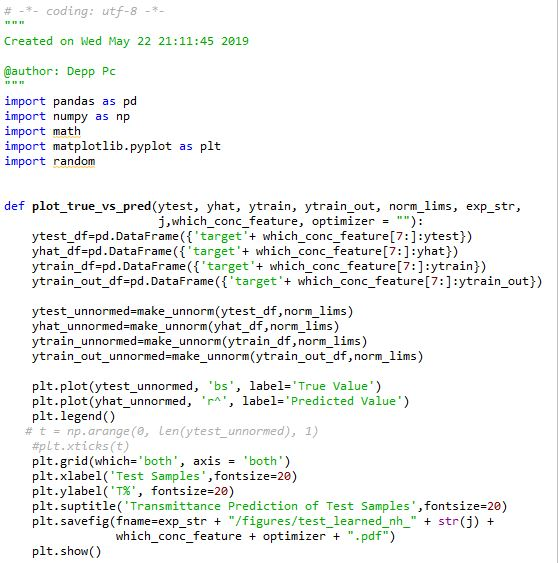
\includegraphics[width=1\textwidth,height=\textheight]{images/utility1.jpg}
\end{figure}

\begin{figure}
\centering
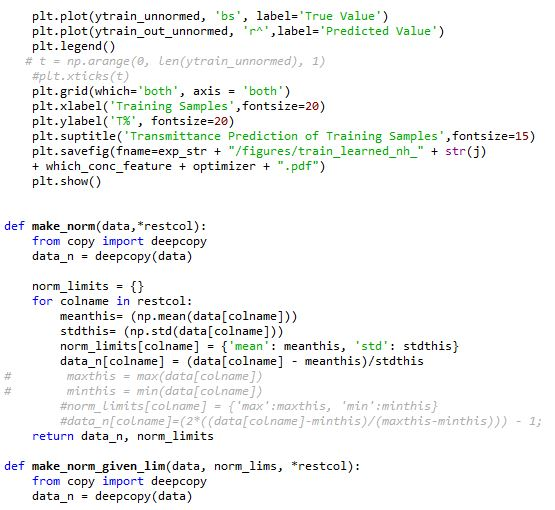
\includegraphics[width=1\textwidth,height=\textheight]{images/utility2.jpg}
\end{figure}

\begin{figure}
\centering
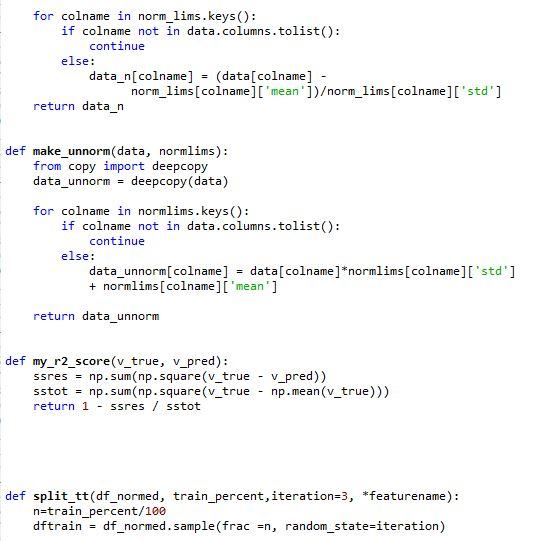
\includegraphics[width=1\textwidth,height=\textheight]{images/utility3.jpg}
\end{figure}

\begin{figure}
\centering
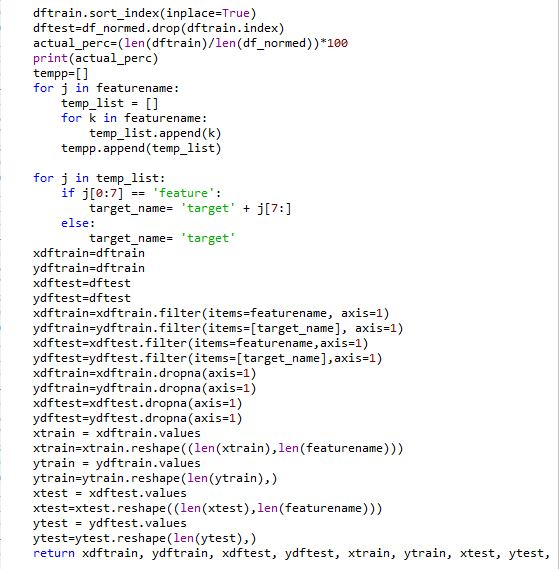
\includegraphics[width=1\textwidth,height=\textheight]{images/utility4.jpg}
\end{figure}


\hypertarget{utitlity-flann}{%
\subsection{Utitlity FLANN Code}\label{utitlity-flann}}


\begin{figure}
\centering
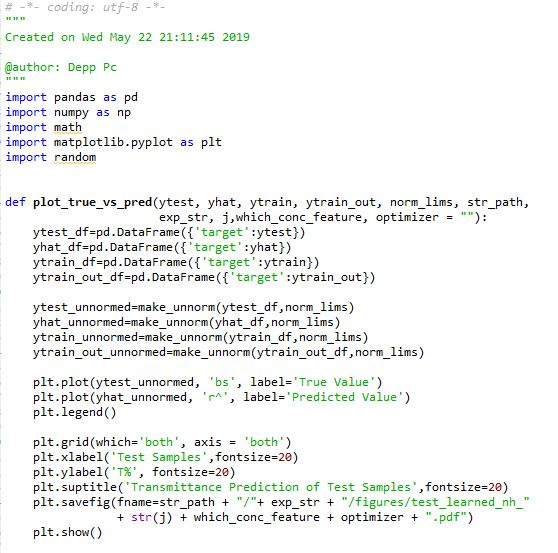
\includegraphics[width=1\textwidth,height=\textheight]{images/utilityflann1.jpg}
\end{figure}

\begin{figure}
\centering
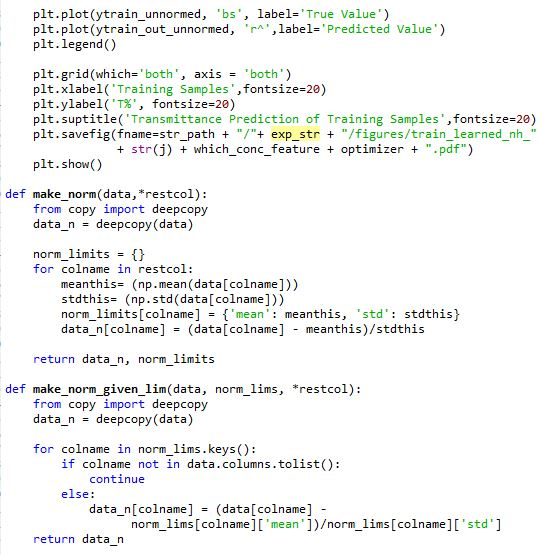
\includegraphics[width=1\textwidth,height=\textheight]{images/utilityflann2.jpg}
\end{figure}
\begin{figure}
\centering
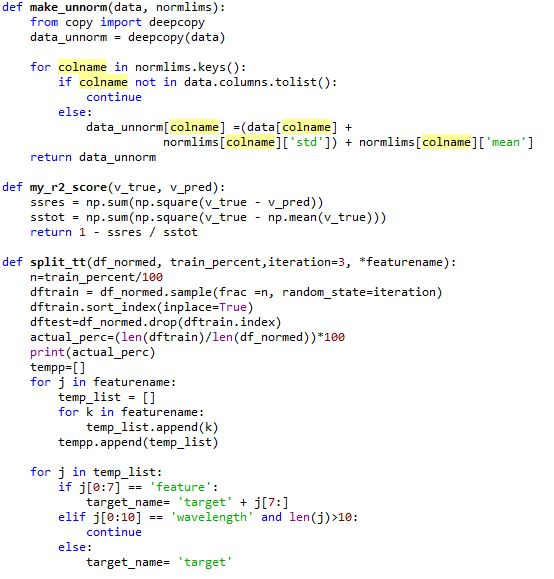
\includegraphics[width=1\textwidth,height=\textheight]{images/utilityflann3.jpg}
\end{figure}
\begin{figure}
\centering
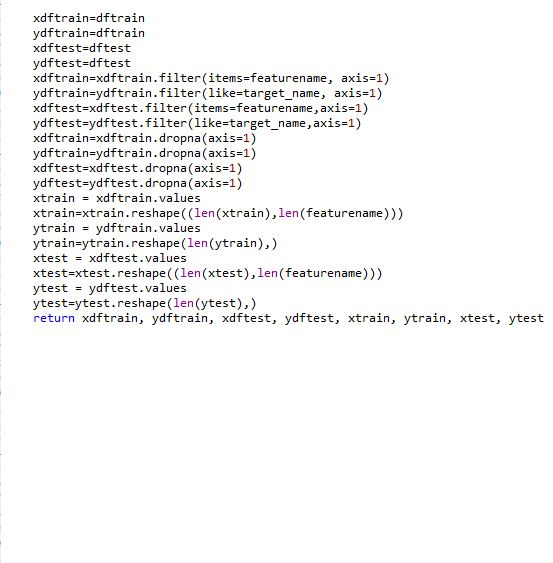
\includegraphics[width=1\textwidth,height=\textheight]{images/utilityflann4.jpg}
\end{figure}

\hypertarget{mlp-code}{%
\subsection{MLP Code}\label{mlp-code}}


\begin{figure}
\centering
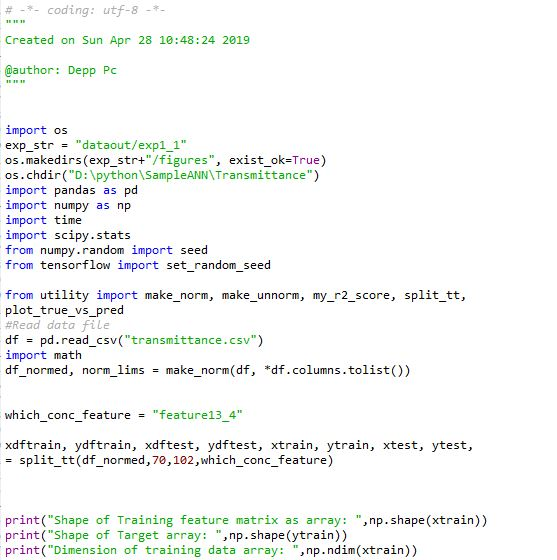
\includegraphics[width=1\textwidth,height=\textheight]{images/mlp1.jpg}
\end{figure}

\begin{figure}
\centering
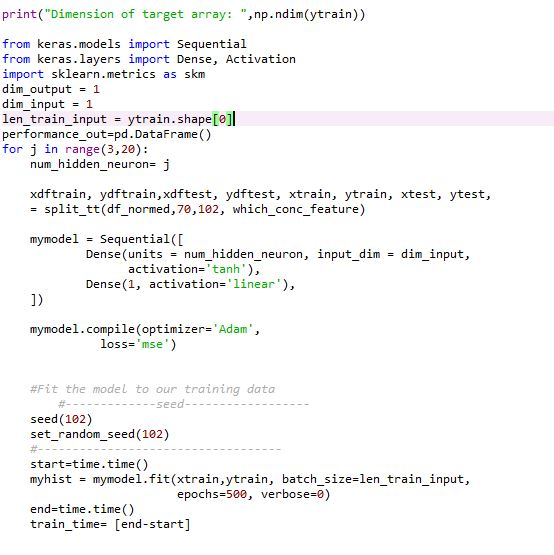
\includegraphics[width=1\textwidth,height=\textheight]{images/mlp2.jpg}
\end{figure}

v

\begin{figure}
\centering
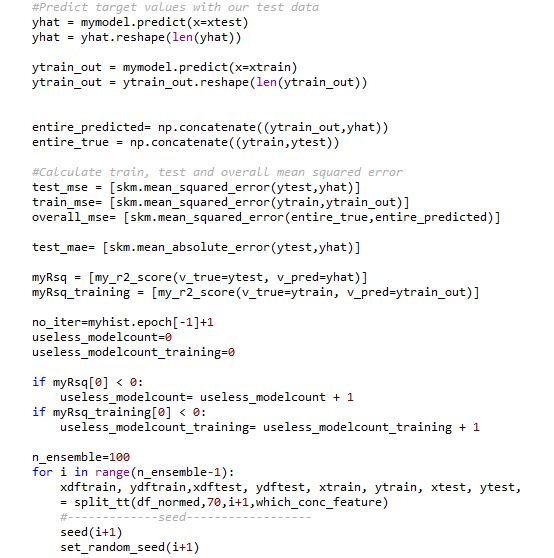
\includegraphics[width=1\textwidth,height=\textheight]{images/mlp3.jpg}
\end{figure}

\begin{figure}
\centering
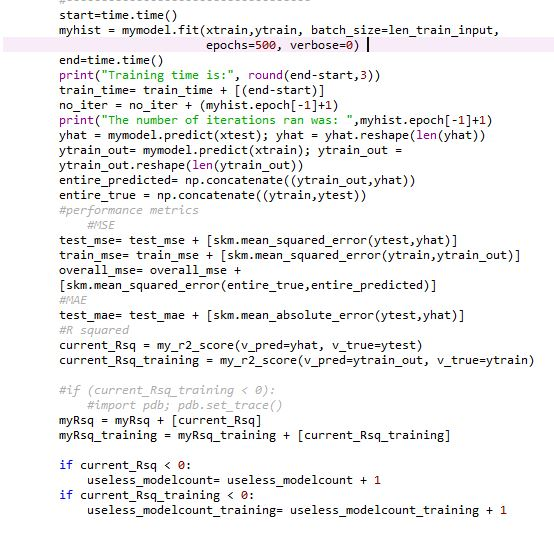
\includegraphics[width=1\textwidth,height=\textheight]{images/mlp4.jpg}
\end{figure}

\begin{figure}
\centering
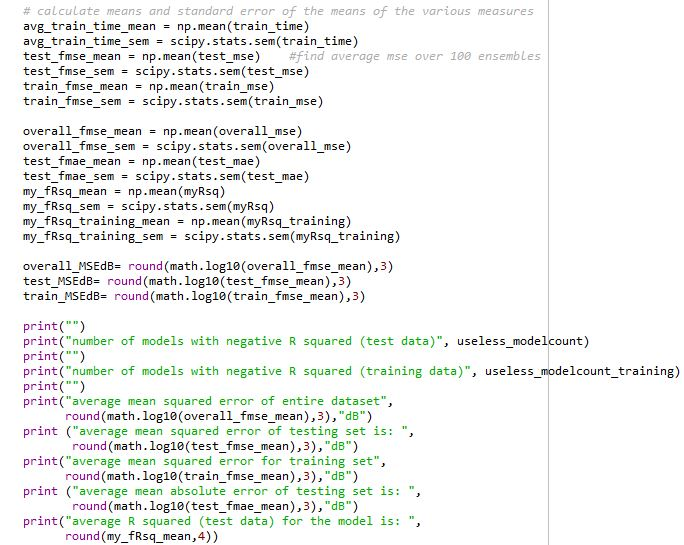
\includegraphics[width=1\textwidth,height=\textheight]{images/mlp5.jpg}
\end{figure}

\begin{figure}
\centering
\includegraphics[width=1\textwidth,height=\textheight]{images/mlp6.jpg}
\end{figure}

\begin{figure}
\centering
\includegraphics[width=1\textwidth,height=\textheight]{images/mlp7.jpg}
\end{figure}


\hypertarget{flann-code}{%
\subsection{FLANN Code}\label{flann-code}}


\begin{figure}
\centering
\includegraphics[width=1\textwidth,height=\textheight]{images/flann1.jpg}
\end{figure}


\begin{figure}
\centering
\includegraphics[width=1\textwidth,height=\textheight]{images/flann2.jpg}
\end{figure}

\begin{figure}
\centering
\includegraphics[width=1\textwidth,height=\textheight]{images/flann3.jpg}
\end{figure}

\begin{figure}
\centering
\includegraphics[width=1\textwidth,height=\textheight]{images/flann4.jpg}
\end{figure}

\begin{figure}
\centering
\includegraphics[width=1\textwidth,height=\textheight]{images/flann5.jpg}
\end{figure}

\begin{figure}
\centering
\includegraphics[width=1\textwidth,height=\textheight]{images/flann6.jpg}
\end{figure}

\begin{figure}
\centering
\includegraphics[width=1\textwidth,height=\textheight]{images/flann7.jpg}
\end{figure}

\begin{figure}
\centering
\includegraphics[width=1\textwidth,height=\textheight]{images/flann8.jpg}
\end{figure}


\end{document}
